\documentclass[../appunti-analisi.tex]{subfiles}

\begin{document}

\section{Calcolo infinitesimale per le curve}

\subsection{Calcolo vettoriale}

\subsubsection{Vettori}

\defn{Vettore}{ Il vettore \(\ux \in \Rn \) è una n-upla \(\ux=(x_1,x_2, \ldots,x_n)\) }

In genere i vettori si indicano con \(\ux \) o \(\vec{x}\) o \(\overline{x}\), per indicare che sono variabili a più valori.

\subsubsection{Funzioni in più variabili}

In particolare:

\begin{itemize}
    \item \(f: A \in \Rn  \rightarrow \R \)
    \item \(g: A \in \Rn \rightarrow \R^{m}\)
\end{itemize}

Noi ci occuperemo solo di funzione reali di più variabili, ovvero funzioni da \(\Rn \to \R \)

\subsubsection*{Operazioni in \(\Rn \)}

\begin{itemize}
    \item Moltiplicazione per uno scalare reale:

          \[
              \forall c \in \R, \quad \forall \ux \in \Rn
          \]
          \[
              c \cdot \ux = (cx_1, \ldots ,cx_n)
          \]

    \item Somma:

          \[
              \forall \ux, \uy  \in \Rn
          \]
          \[
              \ux  =(x_1, \ldots ,x_n), \quad \uy  = (y_1, \ldots ,y_n)
          \]
          \[
              \ux+ \uy = (x_1+y_1, \ldots ,x_n+y_n)
          \]

\end{itemize}

\pagebreak{}

\subsubsection{Prodotto scalare}

L'operazione \(\prods{}{} : \Rn \times \Rn \rightarrow \R \)

\[
    \forall \ux ,\uy \in \Rn
\]
\[
    \prods{\ux}{\uy} := \ux \bullet \uy := \sum^{n}_{i=1} x_i y_i
\]

\subsubsection*{Esempio}
\[
    \ux=(1,2,0,3,5) \in \R^{5}
\]
\[
    \uy=(2,5,1,7,3) \in \R^{5}
\]
\[
    \prods{\ux}{\uy} = (1\cdot2)+(2\cdot5)+(0\cdot1)+(3\cdot7)+(5\cdot3) = 48
\]

\subsubsection*{Proprietà}

Il prodotto scalare verifica le seguenti proprietà

\begin{enumerate}
    \item \textbf{Bilinearità} (lineare su ogni fattore):

          \[
              (\alpha \ux_1 + \beta \ux_2) \bullet \uy = \prods{(\alpha \ux_1 + \beta \ux_2)}{\uy} = \alpha \prods{\ux_1}{\uy} + \beta \prods{\ux_2}{\uy}
          \]

          \[
              \forall \ux_1,\ux_2,\uy \in \R, \quad \forall \alpha, \beta \in \R
          \]

    \item \textbf{Simmetria} (l'ordine non conta)

          \[
              \forall \ux,\uy \in \Rn
          \]
          \[
              \prods{\ux}{\uy} = \prods{\uy}{\ux}
          \]

    \item \textbf{Positività}

          \[
              \forall \ux \in  \Rn
          \]
          \[
              \ux=(x_1, \ldots ,x_n)
          \]
          \[
              \prods{\ux}{\ux} = \sum^{n}_{i=1} {x_i}^{2}\ge 0
          \]
          \[
              \prods{\ux}{\ux} = 0 \iff \ux = \uzero = (0, \ldots ,0)\ \text{vettore nullo}
          \]

\end{enumerate}

\filbreak{}

\subsubsection{Norma di un vettore e proprietà associate}

\defn{Norma}{
    Il numero reale (non negativo)

    \[
        \norm\ux := \sqrt{\prods{\ux}{\ux}} := \sqrt{\sum_{i=1}^{n} {(x_i)}^2} \qquad (\ge 0)
    \]

    si chiama \textbf{lunghezza} o \textbf{norma} del vettore.

    Si può trovare anche scritta come \(|\ux|\), ma questa notazione è sconsigliata in quanto collide con quella di valore assoluto e quella di determinante.
}

\proposizione{Formula di Carnot}{

    \[
        \forall \ux,\uy \in \Rn
    \]
    \[
        \norm{\ux+\uy}^{2} = \norm\ux^{2} + \norm\uy^{2} + 2\prods{\ux}{\uy}
    \]
}

\begin{proof}
    \begin{align*}
        \norm{\ux+\uy} ^{2}  & = \langle \ux+\uy , \ux+\uy \rangle                                                       \\
        \text{(bilinearità)} & = \langle \ux,\ux+\uy \rangle + \langle \uy,\ux+\uy \rangle                               \\
        \text{(bilinearità)} & = \prods{\ux}{\ux} + \prods{\ux}{\uy} + \langle \uy,\ux \rangle + \langle \uy,\uy \rangle \\
                             & = \prods{\ux}{\ux} + 2\prods{\ux}{\uy} + \langle \uy,\uy \rangle                          \\
                             & = \norm\ux^{2} + \norm\uy^{2} + 2 \langle\ux, \uy\rangle
    \end{align*}

\end{proof}

\subsubsection*{Osservazione}

\(
\norm{\ux+\uy}^{2}= \norm\ux^{2} + \norm\uy^{2} \iff \langle \ux, \uy \rangle  =0
\)

\proposizione{Disuguaglianza di Cauchy-Schwarz}{
    \[
        \forall \ux,\uy \in \Rn
    \]
    \begin{align*}
        \circled{1} \qquad & |\prods{\ux}{\uy}| \le \norm\ux\cdot \norm\uy    &                                                                         \\
        \circled{2} \qquad & |\prods{\ux}{\uy}| = \norm\ux\cdot \norm\uy \iff &   & \uy = 0 \lor \ux=\lambda \uy \quad \text{ con } \lambda \in \R\ge 0 \\
                           &                                                  &   & \text{se e solo se un vettore è multiplo scalare dell'altro}
    \end{align*}
}

Vediamo ora le dimostrazione di queste due proprietà:

\begin{proof} di \(\circled{1}\)

    Se \(\uy = \uzero = (0, \ldots ,0)\) la testi è ovvia;

    Sia dunque \(\Rn  \rightarrow \uy \neq 0\) e consideriamo la funzione reale di una variabile reale \(t \rightarrow \norm{\ux+t\uy}^{2}\ge 0\) polinomio di secondo grado in t

    \begin{align*}
        ||\ux + t\uy|| ^{2} & \overset{\text{Carnot}}{=} \norm\ux^{2} + ||t\uy||^{2} + 2\langle \ux,t\uy \rangle \\
                            & = \norm\ux^{2} + \norm\uy^{2}t^{2} + 2 \prods{\ux}{\uy} t \ge 0
    \end{align*}

    è un polinomio di II grado in t dove \(\norm\uy^{2}> 0 \) essendo \(\uy \neq 0\) per ipotesi

    Il nostro \(\frac{\Delta}{4}\) deve essere negativo (sennò in qualche punto il polinomio dovrebbe essere negativo ma abbiamo supposto che sia sempre positivo):

    \begin{align*}
        \frac{\Delta}{4} = {\prods{\ux}{\uy}}^{2} - \norm\ux^{2}\norm\uy^{2} & \le 0                                       \\
        {\prods{\ux}{\uy}}^{2}                                               & \le \norm\ux^{2}\norm\uy^{2}                \\
        \prods{\ux}{\uy}                                                     & \le \norm\ux \norm\uy \quad (= \text{tesi})
    \end{align*}

\end{proof}

\filbreak{}

\begin{proof} di \(\circled{2}\)

    Si verifica, se si ha che

    \[
        \prods{\ux}{\uy} = \norm\ux \cdot \norm\uy
    \]

    si ha che il \(\Delta \) del trinomio di II grado è nullo e dunque \(\exists t \in \R \) per cui
    \[\norm{\ux+t\uy}^{2}=0 \implies \ux +t\uy=0 \implies \ux=-t\uy \]

    devo mostrare che \(-t \ge 0\)

    \[
        t = - \frac{\prods{\ux}{\uy}}{\norm\uy^{2}}
    \]

    si ricorda che \(\norm\uy>0\) essendo \uy{} non nullo

    \[
        -t = \frac{\norm\ux \cdot \norm\uy}{\norm\uy^{2}}\ge 0
    \]

\end{proof}

\filbreak{}

\subsubsection{Funzione ``lunghezza'' di un vettore}

Definiamo ora la funzione \textbf{lunghezza} di un vettore.

\begin{align*}
    \text{len}(\ux): \ \Rn & \rightarrow \R_0^{+}            \\
    \ux                    & \mapsto \norm\ux \quad (\geq 0)
\end{align*}

La funzione lunghezza è una norma, ovvero, \(\forall \ux \in \Rn , \quad \forall \lambda \in \R \):

\begin{enumerate}
    \item \(\norm\ux \in \R, \quad \norm\ux \geq 0\)
    \item \(\norm\ux = 0 \iff \ux = 0\)
    \item \(\norm{\lambda \ux} = |\lambda| \cdot \norm\ux \) \hfill (omogeneità)
    \item \(\norm{\ux+\uy} \leq \norm\ux + \norm\uy \) \hfill (disuguaglianza triangolare)
\end{enumerate}

\defn{Disuguaglianza triangolare}{
    La disuguaglianza triangolare si definisce come:

    \[
        \norm{\ux+\uy} \le \norm\ux+\norm\uy
    \]

    se \(\norm{\ux+\uy} = \norm\ux + \norm\uy \implies \uy =0 \lor \ux= \lambda \uy \qquad \text{con}\ \lambda \ge 0\):

}

\begin{proof}
    Dimostriamo la disuguaglianza triangolare, consideriamo:

    \begin{align*}
        \norm{\ux+\uy}^{2} & = \prods{\ux+\uy}{\ux+\uy}                                                                             \\
                           & = \norm\ux^{2}+\norm\uy^{2} + 2 \prods{\ux}{\uy}                                                       \\
                           & \le \norm\ux^{2} + \norm\uy ^{2} + 2|\prods{\ux}{\uy}|                                                 \\
                           & \le \underbrace{\norm\ux ^{2} + \norm\uy^{2} + 2(\norm\ux \cdot \norm\uy)}_{{(\norm\ux+\norm\uy)}^{2}}
    \end{align*}

    estraendo e passando alle radici si ha

    \[
        \norm{\ux+\uy} \le \norm\ux+\norm\uy
    \]
\end{proof}


\newpage
\subsection{Spazio metrico}

\subsubsection{Distanza Euclidea}

\defn{Distanza Euclidea}{
Si definisce distanza euclidea tra \(\ux \) e \(\uy \) il numero reale non negativo definito da:

\[
    d(\ux,\uy) := \norm{\ux-\uy} = \sqrt{\prods{\ux-\uy}{\ux-\uy}} = \sqrt{\sum^n_{i=1} {(x_i - y_i)}^2}\ \ge 0
\]
\[
    d: \Rn \times \Rn \to \R^+_0
\]
}

La distanza euclidea verifica le proprietà della distanza:

\begin{enumerate}
    \item \(d(\ux,\uy) \ge 0, \quad d(\ux,\uy) \in \R \)
    \item \(d(\ux,\uy) = 0 \iff \ux =\uy \)
    \item \(d(\ux,\uy) = d(\uy,\ux)\) \hfill (simmetria)
    \item \(d(\ux,\uy) \le d(\ux,\underline{z}) + d(\underline{z},\uy),\ \ \forall \, \ux,\uy,\underline{z} \in \Rn \) \hfill (disuguaglianza triangolare)
\end{enumerate}

\subsubsection{Definizione di spazio metrico}

\defn{Spazio metrico}{
    Si definisce spazio metrico un insieme della forma \(X, d\) con, \(X\) insieme, e \(d: X \times X \to \R^+_0\) un'applicazione che soddisfa le proprietà della distanza.

    Un esempio è il seguente:

    \[
        (\Rn ,d) \quad \text{con}\ d= \text{distanza euclidea}
    \]
}

Anche se noi useremo solo la distanza euclidea come metrica, esistono altri tipi di distanze con le quali è possibile definire rispettivi spazi metrici. Vediamone un paio:

\subsubsection*{Distanza Taxicab (o Manhattan)}

\[
    \ux=(x_1,x_2),\ \uy=(y_1,y_2) \quad \forall \ux,\uy \in \R^2
\]
\[
    d_1(\ux,\uy) = |y_1-x_1| + |y_2-x_2|
\]

\subsubsection*{Distanza di Chebyshev (o degli scacchi)}

\[
    \ux=(x_1,x_2),\ \uy=(y_1,y_2) \quad \forall \ux,\uy \in \R^2
\]
\[
    d_2(\ux,\uy) = \max \{ |y_1-x_1|,\ |y_2-x_2| \}
\]

\filbreak{}

\subsubsection{Successioni convergenti in \texorpdfstring{\(\Rn{}\)}{Rn}}

\defn{Successione in \(\Rn \)}{
    Una successione a valori in \(\Rn \) è una successione del tipo:
    \[
        {\{{\ux}_n\}}_{\N} \subset \Rn
    \]
    Ogni elemento di questa successione è un insieme ordinato di \(n\) numeri reali:
    \[
        {\ux}_n = (x_n^1, x_n^2, \ldots, x_n^n)\ \in \Rn
    \]
    La notazione abbreviata della successione è: \( \{{\ux}_n\} \)
}

\defn{Convergenza di una successione in \(\Rn \)}{
Si dice che una successione \( \{{\ux}_n\} \) converge a \(\ux = (x_1, x_2, \ldots, x_n) \in \Rn \) se:

\[
    \lim_{n \to +\infty} d({\ux}_n,\ux) = 0
\]

ovvero:
\begin{align*}
    \forall \varepsilon >0,\ \exists \bar{N} \in \N
    \giventhat[\Big]
    d(\ux_n, \ux ) < \varepsilon ~\forall n \ge \bar{N}
\end{align*}

questo significa che:
\[
    d(\ux_n, \ux ) = \norm{\ux_n - \ux} = \sqrt{{(x_n^1-x_1)}^2 + \cdots + {(x_n^n-x_n)}^2}
\]
tende a 0 per \(n \to +\infty \iff (x_{n}^{i} - x_{i}) = 0 \quad \forall i = 1 \cdots n \)
}

\proposizione{}{ Sia \( \{\ux_n\} \subset \Rn \) una successione in \(\Rn \). Si ha:

    \begin{enumerate}
        \item (\textbf{Unicità}) Se \( \{\ux_n\} \) ammette limite, allora questo è unico
        \item (\textbf{Limitatezza}) Ogni successione convergente è limitata, ovvero:

              \[
                  \exists \ux_0 \in \Rn ,\ M \in \R
                  \giventhat[\Big]
                  d(\ux_n,\ux_0) \le M \quad \forall n \in \N
              \]

        \item (\textbf{Sottosuccessione}) Se \( \{\ux_n\} \to \ux \) in \(\Rn \) allora ogni sua sottosuccessione \( \{\ux_{n_k}\} \) di \( \{\ux_n\} \) converge allo stesso limite (\(\ux \))
    \end{enumerate}

}

\pagebreak{}

\subsubsection{Elementi di topologia in \texorpdfstring{\(\Rn \)}{Rn}}

Sia \(\ux_0 \in \Rn \) fissato e \(\R \ni r>0\)

Si ha la seguente definizione

\defn{}{Si definisce \textbf{palla aperta}, o \textbf{disco aperto}, o \textbf{intorno sferico di centro} \(\ux_0\) \textbf{e raggio} \(r\) l'insieme che si indica con:

    \[
        B(\ux_0,r) := \{ \ux \in \Rn \giventhat d(\ux,\ux_0)<r\} \subset \Rn
    \]
}

\subsubsection*{In n=1}

\(x_0 \in \R, \quad r > 0\)

\(B(x_{0},r) = x \in \left( x_0-r,\ x_0+r \right)\)

\subsubsection*{In n=2}

\begin{center}
    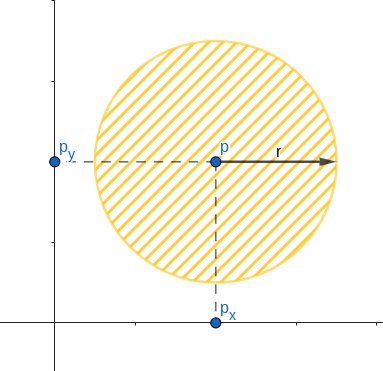
\includegraphics[scale=0.5]{intorno-sferico-r2.png}
\end{center}

\subsubsection*{In n=3}

\begin{center}
    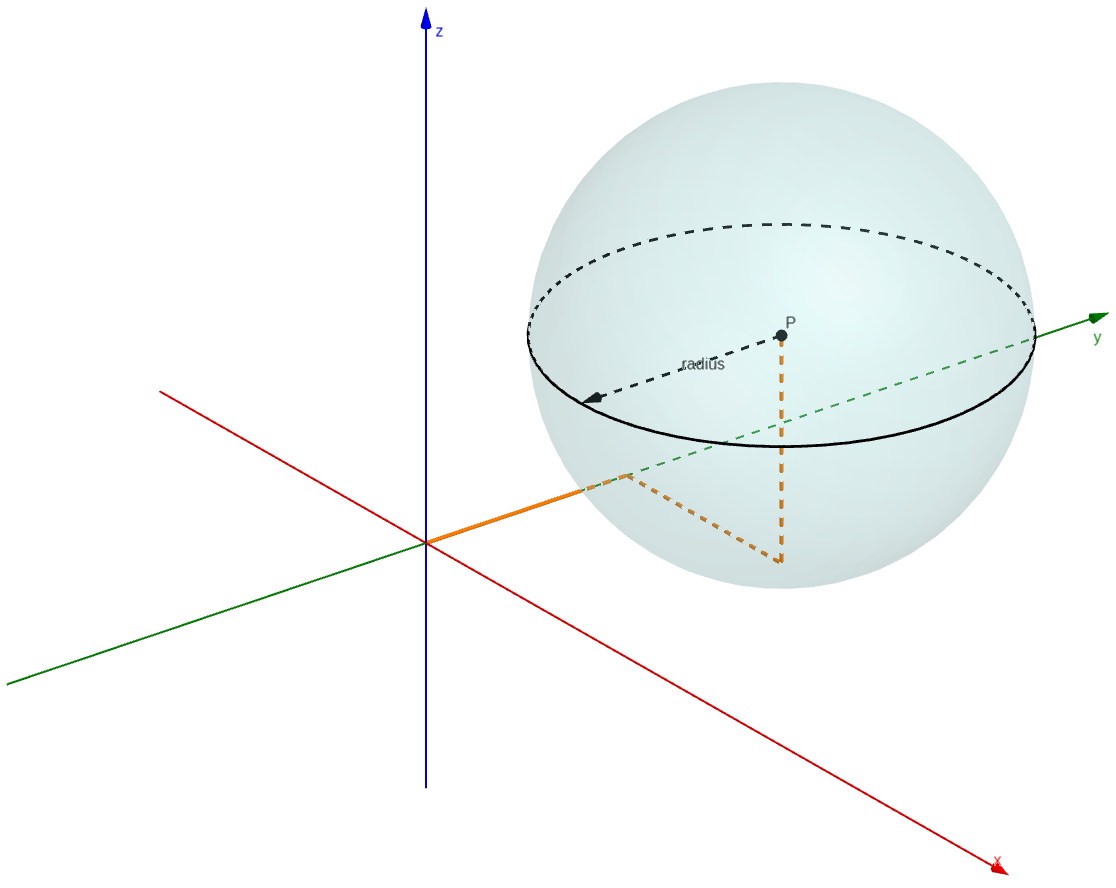
\includegraphics[width=\textwidth/2]{intorno-sferico-r3.png}
\end{center}

\filbreak{}

\subsubsection*{Esempio con distanza Euclidea e Taxicab}

Ricordando che con \(d\) si indica la distanza Euclidea e che con \(d_1\) si indica la distanza Taxicab; si ha la seguente situazione:

\[
    (\R^{2},d) \rightarrow d(\ux,\uy) = \sqrt{\sum^{r}_{i=1} {(x_i-y_i)}^2}
\]

\[
    (\R^{2},d_1) \rightarrow d_1(\ux,\uy) = |x_1-y_1| + |x_2-y_2|
\]

\vspace{6mm}
Definito un centro, \(x_0=0\), e un raggio, \(r=1\), con la distanza Euclidea si ha:

\[
    B(\uzero,1) = \{\ux \in \R^2 \giventhat d(\ux,\uzero) <1\} = \{\ux \in \R^2 \giventhat \sqrt{{x_1}^2+{y_1}^2}<1\}
\]

\begin{center}
    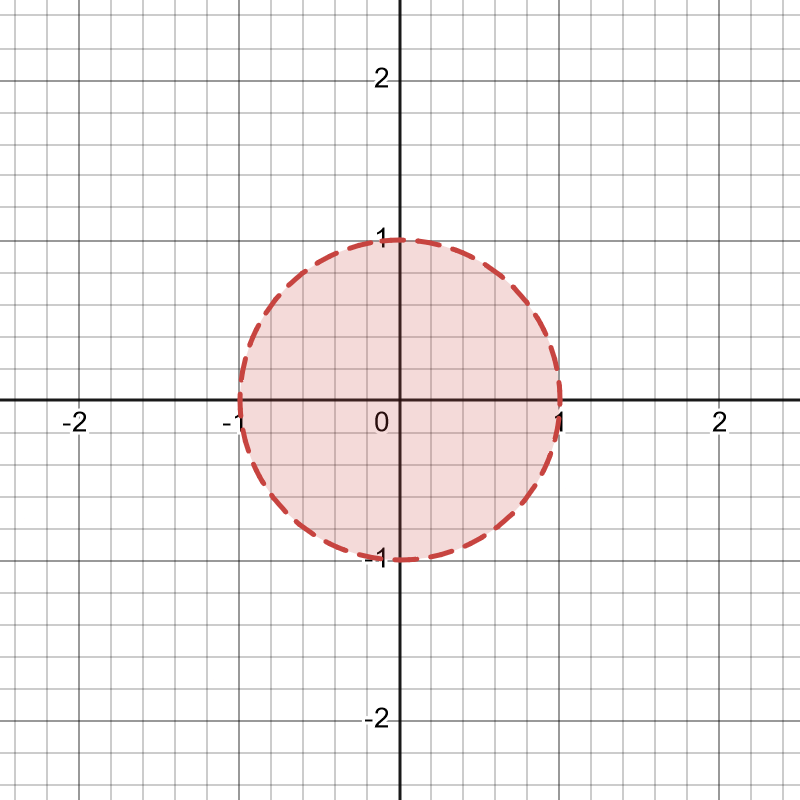
\includegraphics[width=0.32\textwidth]{distanza-euclidea-esempio.png}
\end{center}

mentre con la distanza Taxicab si ha:

\[
    B(\uzero,1) = \{\ux \in \R^2 \giventhat d_1(\ux,\uzero) <1\} = \{\ux \in \R^2 \giventhat \underbrace{|x_1-0|}_{x_1} + \underbrace{|y_1-0|}_{y_1}<1\}
\]

\begin{center}
    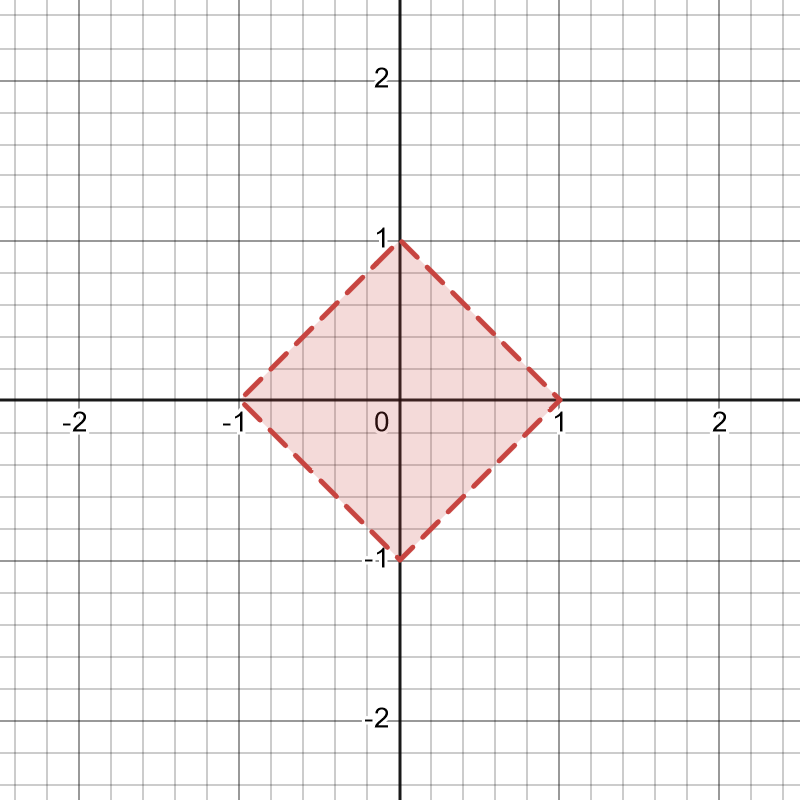
\includegraphics[width=0.32\textwidth]{distanza-taxicab-esempio.png}
\end{center}

\pagebreak

\subsubsection{Convergenza di successioni in uno spazio metrico}

Attraverso gli intorni sferici possiamo ridefinire il concetto di convergenza di successioni (limite) visto in precedenza.

\begin{align*}
    \{\ux_n\} \subset \Rn \text{ converge a } \ux_0 \in \Rn
    \iff
    \forall \varepsilon >0 ~\exists N_\varepsilon \in \N
    \giventhat[\Big]
    \ux_n \in B\left(\ux_0,\varepsilon\right) ~\forall n \ge N_\varepsilon
\end{align*}

\(
\ux_n \in B\left(\ux_0,\varepsilon\right) \implies \ux_n \text{ appartiene all'intorno sferico di centro } \ux_0 \text{ e raggio } \varepsilon
\)

\pagebreak

\subsubsection{Limitatezza in uno spazio metrico}

\defn{Insieme limitato}{
    \(A \subset X\) si dice \textbf{limitato} se esiste una palla aperta in cui \(A\) risulta interamente contenuto:

    \[
        \exists r>0,x_0 \in X \giventhat[\Big] A \subset B(x_0,r)
    \]

    e.g.{:} in \(X = \Rn \) con \(\ux_{0} = (0,0)\), \(A\) è limitato se è contenuto in un intorno sferico dell'origine, ovvero:

    \[
        \exists M > 0 \giventhat \norm{\ux} < M ~\forall \ux \in A
    \]
}

\defn{Punto interno}{
    Un punto di \(x_0 \in X\) si dice \textbf{interno} ad \(A\), con \(A \subset X\), se \(x_0 \in A\) e se esiste almeno un suo intorno sferico interamente contenuto in \(A\), ovvero:

    \[
        \exists r>0 \giventhat B(x_0,r) \subset A
    \]

    \(\mathring{A} =\) insieme dei punti interni di \(A\)
}

\defn{Punto esterno}{
    \(x_0 \in X\) si dice \textbf{esterno} ad \(A\) (\(A \subset X\)) se \(x_0 \notin A\) ed esiste almeno un suo intorno sferico completamente disgiunto da \(A\)

    \[
        \exists r>0 \giventhat[] B(x_0,r) \cap A = \emptyset
    \]
}

\defn{Punti di frontiera}{
    La frontiera di A si indica con il simbolo: \(\frontiera{A}\).

    I punti che non sono ne esterni, ne interni ad A, costituiscono la \textbf{frontiera} di A.
    Quindi, \(x_{0} \in \frontiera{A}\) se ogni suo intorno sferico contiene sia punti interni che punti esterni ad \(A\).
}

\defn{Punto di accumulazione}{

    Sia \(A \subseteq \Rn \) e sia \(\ux_0 \in \Rn \).

    Il punto \(\ux_0\) si dice, di \textbf{accumulazione} per \(A\), se ogni intorno sferico di \(\ux_0\) contiene almeno un punto di \(A\) diverso da \(\ux_0\), ovvero:

    \[
        \forall r > 0 \quad B(\ux_{0},r) \cap (A \setminus \{\ux_{0}\}) \neq \emptyset
    \]

    L'insieme dei punti di accumulazione di A si indica con il simbolo: \(D(A) = DA\)

    Esempi:
    \begin{itemize}
        \item I punti che costituiscono l'insieme dei punti interni di \(A = \mathring{A}\), sono punti di accumulazione
        \item I punti di frontiera, ovvero i punti di \(\frontiera{A}\) possono essere punti di accumulazione di \(A\) oppure no. Se il punto di frontiera non è di accumulazione, si chiama \textbf{punto isolato}.
    \end{itemize}
}

\defn{Chiusura di un insieme}{
    \textbf{Chiusura} di \(A \subset \Rn = \bar{A} = \mathring{A} \cup \frontiera{A} \qquad \) (interni + frontiera)

    Si può inoltre dimostrare che: \(\bar{A} = A \cup DA\)
}

\defn{Insieme aperto}{
    \(A \subset X\) si dice \textbf{aperto} se \(\mathring{A} = A\).

    E.g.: \(A \subset X\) è aperto se \(A = \emptyset \) oppure se ogni punto è un punto interno di \(A\).
}

\defn{Insieme chiuso}{
    Un insieme \(C \subset X\) si dice \textbf{chiuso} se contiene tutti i suoi punti di frontiera, ovvero, \(\frontiera{C} \subset C\)
}

\defn{Dominio}{
    Un dominio \(D\) in \(\Rn \) è la chiusura di un insieme aperto:

    \[
        D = \bar{A}  = A \cup \frontiera{A} \quad \text{con } A \text{ aperto}
    \]

    E.g.{:} in \(\Rn \) una sfera chiusa è un dominio: \( \{ \ux \in \Rn \giventhat \norm{\ux} \le M \} \) con \(M \in \N \) fissato.
}

\subsubsection*{Esempi di insiemi aperti}

\(A_1= \{ (x,y) \in \R^2 \giventhat x \neq y^2\} \)

\vspace{2mm}\hspace{6mm}
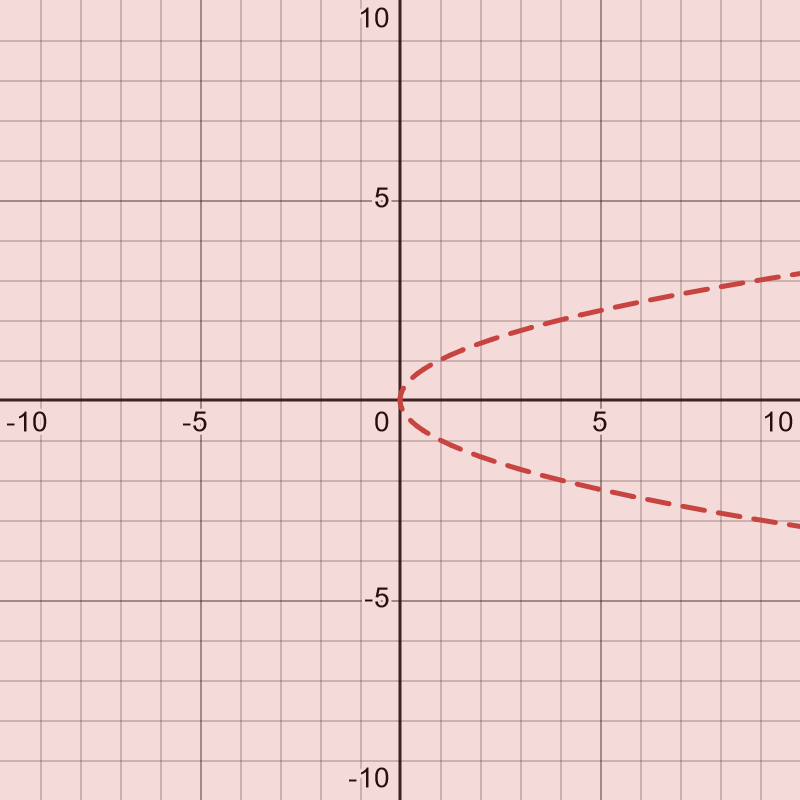
\includegraphics[width=0.33\textwidth]{insiemi-aperti-esempio-1.png}
\vspace{8mm}

\(A_2= \{ (x,y) \in \R^2 \giventhat x^2+ y^2 < 25\} \)

\vspace{2mm}\hspace{6mm}
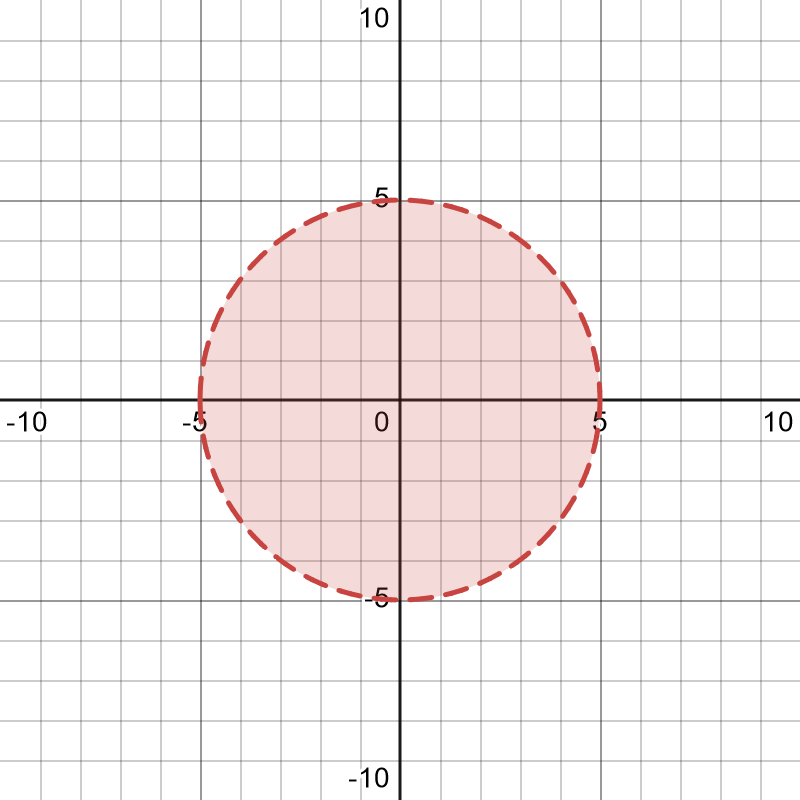
\includegraphics[width=0.33\textwidth]{insiemi-aperti-esempio-2.png}
\vspace{8mm}

\(A_3= \{ (x,y) \in \R^2 \giventhat x^2+ 2y +1 \le 0\} \)

\vspace{2mm}\hspace{6mm}
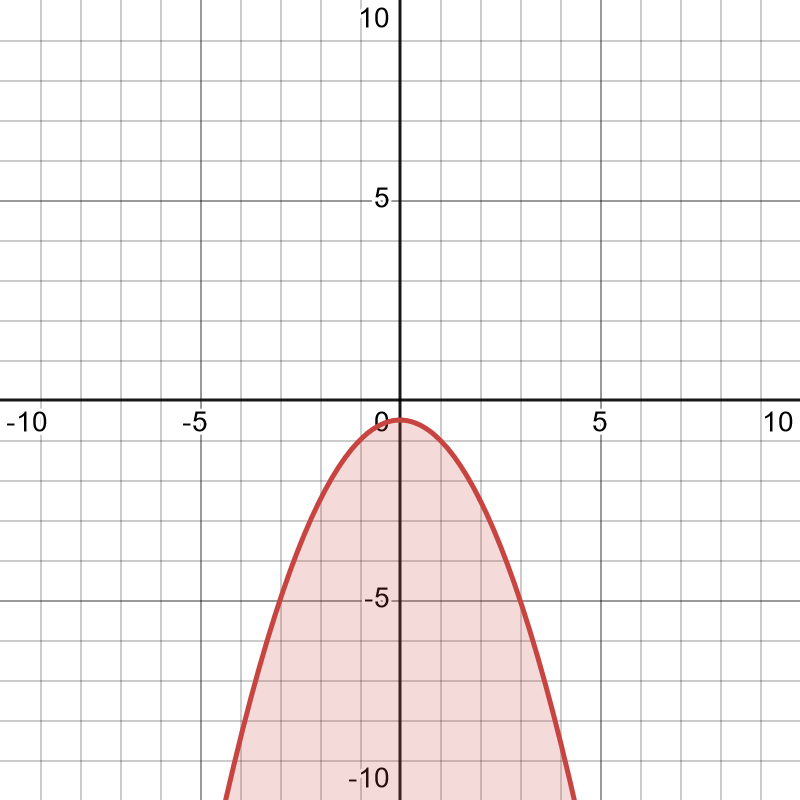
\includegraphics[width=0.33\textwidth]{insiemi-aperti-esempio-3.png}
\vspace{8mm}

\newpage
\subsection{Limiti e Continuità di funzioni in più variabili}

\subsubsection{Definizione di limiti per funzioni a più variabili}

\defn{Convergenza in \(\Rn \)}{
    Data una successione \( \{\ux_n\}\in \Rn \) questa si dice che converge a \(\ux_0 \in  \Rn \) se:

    \[
        \lim_{ n \to +\infty } d(\ux_n,\ux_0)=0
    \]

    questo equivale a dire:

    \[
        \forall \varepsilon >0 ~\exists \bar{n} \in \N \giventhat d(\ux_n,\ux_0) < \varepsilon ~\forall n \ge \bar{n}
    \]

}

\defn{Punto di accumulazione con limiti}{

    \(\ux_0\) è punto di accumulazione per \(A\) \(\iff \ux_0\) è il limite di una successione di elementi di \(A\) tutti diversi da \(\ux_0\)
}

\filbreak{}

\subsubsection*{Esempio di punti di accumulazione}

Determinare i punti di accumulazione e di frontiera dell'insieme seguente, \(A\), e stabilire se \(A\) è aperto o chiuso.

\[
    A = \{\ux \in \R^{2} \giventhat 2 < \norm{\ux} < 3 \}
\]

dove \(\ux=(x,y)\) e \(\norm{\ux} = d(\ux,\uzero) = \sqrt{x^{2}+y^{2}}\)
\begin{center}
    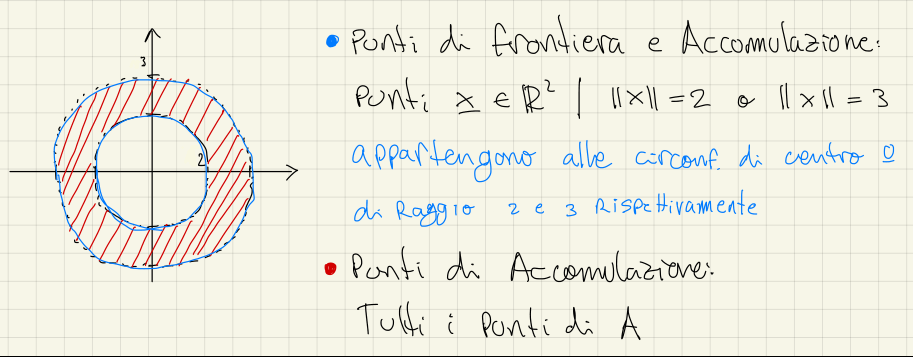
\includegraphics[width=\textwidth-2cm]{disegno-punti-di-accumulazione-esempio.png}
\end{center}

\filbreak{}

\defn{Limite di funzioni in più variabili}{
    Consideriamo ora le funzioni in più variabili
    \[f: A \subset \Rn \rightarrow \R \]
    Sia \(\ux_0 \in \Rn \) un punto di accumulazione per \(A\). Si scrive:

    \[
        \lim_{ \ux  \to \ux_0 } f(\ux ) = l
    \]

    \begin{itemize}
        \item Se \(l \in \R \cup \{ \pm \infty \} \):

              si dice che \(f(\ux)\) tende a \(l\) per \(\ux \) che tende a \(\ux_0\)

              se \(\forall \) intorno \(U \subset \R \) di \(l\) esiste un intorno sferico di \(\ux_0\), \(I(\ux_0,r)\) con \(r>0\),

              tale che \(f(\ux) \in U ~\forall \ux \in I(\ux_0,r) \cap \,(A \setminus \{\ux_0\})\)
        \item Se \(\ux,\ux_{0} \in \R^2\), \(l \in \R \):

              \(\forall \varepsilon>0 ~\exists \delta = \delta(\varepsilon) >0\)

              tale che \(d( f(x,y), f(x_{0},y_{0}) ) = \big|f(x,y) - f(x_{0},y_{0})\big| < \varepsilon \)

              \(\forall (x,y) \in \left( A \setminus \{(x_{0},y_{0})\} \right) \cap B((x_{0}, y_{0}), \delta)\)

              ovvero \(\forall (x,y) \in A \giventhat 0 < \norm{(x,y) - (x_0,y_0)} < \delta \)
    \end{itemize}
}

\filbreak{}

\subsubsection{Proprietà dei limiti di funzioni in più variabili}

Adesso parliamo di un po' di proprietà:

\begin{itemize}
    \item Il limite quando esiste è \textbf{unico}
    \item I limiti di \textbf{somme} e di \textbf{prodotti} di funzioni sono dati dalla somma e dal prodotto dei limiti (qualora i limiti esistano e le operazioni siano ben definite)
    \item Il limite del \textbf{quoziente} di due funzioni è il quoziente dei limiti (se definito)
\end{itemize}

\proposizione{}{
    Sia \(f: A \subset \Rn \to \R \);

    Sia \((x_0,y_0)\) punto di accumulazione per \(A\);

    Se vale:

    \[
        \lim_{ (x,y) \to (x_0,y_0) } f(x,y)=l
    \]

    allora, per ogni sottoinsieme \(C\) di \(A\) dove \(P_0=(x_0,y_0)\) è un punto di accumulazione per \(C\), deve valere:

    \[
        \lim_{\begin{smallmatrix} (x,y) \to (x_0,y_0) \\ (x,y) \in C \end{smallmatrix}} f(x,y)=l
    \]
}

\pagebreak

\subsubsection{Esempi di esercizi}

Abbiamo due tipologie di esercizi:

\begin{enumerate}
    \item Ci viene chiesto di analizzare cosa fa la funzione quando tende a un punto di accumulazione.

          In questo caso possiamo applicare la definizione di limite per arrivare a capire cosa succede.
    \item Ci viene chiesto di dimostrare che il limite non esiste.

          In questa tipologia di esercizi abbiamo un limite che non esiste e dobbiamo dimostrare che questa cosa è vera. Per far ciò, bisogna studiare la funzione lungo delle curve apposite lungo le quali il limite tende a valori diversi. Avendo trovato due limiti diversi, possiamo quindi concludere che non esiste per la proprietà di unicità dei limiti.

          Queste curve lungo cui studiare la funzione vanno proposte in base al tipo di funzione che abbiamo. Non c'è una regola generale per trovarle.
\end{enumerate}

\subsubsection*{Esempio 1}

Sia
\[
    f(x,y) = \frac{x^{2}}{\sqrt{x^{2}+y^{2}}}
\]

dove il dominio è \(f: \underbrace{\R^{2}\setminus \{(0,0)\}}_\text{A aperto}\rightarrow \R \)

Il punto \((0,0)\) è punto di accumulazione per \(A\)

Vogliamo vedere che succede quando la funzione tende a questo punto di accumulazione. Dimostriamo che:

\[
    \lim_{ (x,y) \to (0,0) } f(x,y) = 0
\]

ovvero che \(\forall \varepsilon >0 ~\exists \delta >0\) tale che \(|f(x,y) -0| < \varepsilon \) \(\forall (x,y) \in A\) con \(0< \sqrt{x^{2}+y^{2}}<\delta \).

Quindi \(~\forall (x,y) \in A\)

\[
    0 \le f(x,y) = \frac{x^{2}}{\sqrt{x^{2}+y^{2}}} \le \frac{x^{2}+y^{2}}{\sqrt{x^{2}+y^{2}}} \overset{\text{razionalizzo}}{=} \sqrt{x^{2}+y^{2}}
\]

E dunque  \(\forall \varepsilon > 0\) si ha:

\[
    0 \le f(x,y) < \varepsilon \qquad \forall (x,y) \neq (0,0) \giventhat[\Big] \sqrt{x^{2}+y^{2}} < \varepsilon
\]

\filbreak{}
\subsubsection*{Esercizio per casa}

Mostrare che il seguente limite non esiste:

\[
    \lim_{ (x,y) \to (0,0) } \frac{x}{\sqrt{x^{2}+y^{2}}}
\]

Se calcolo la funzione in \(y=0\):

\[
    f(x,0) = \frac{x}{\sqrt{x^{2}}}= \frac{x}{|x|}
\]

questa fa:

\begin{equation*}
    \begin{cases}
        1  & x > 0 \\
        -1 & x < 0
    \end{cases}
\end{equation*}

Il limite quindi non esiste perché ha valori diversi a seconda del caso, mentre dovrebbe essere unico, quindi concludo che non esiste.

\filbreak{}
\subsubsection*{Esercizio 1}

Mostriamo che non esiste il seguente limite:

\[
    \lim_{ (x,y) \to (0,0) } \frac{xy}{x^{2}+y^{2}}
\]

\[
    f: \R^2 \setminus \{(0,0)\} \to \R
\]

Facciamo restrizione lungo l'asse x (\(y=0\)):

\[
    C = \{(x,y) \in \R^2 \giventhat x \neq 0 \land y = 0\}
\]

Su \(C\), \(f(x,0) = 0\), infatti:

\[
    \lim_{\begin{smallmatrix} (x,y) \to (0,0) \\ (x,y) \in C \\ y=0 \end{smallmatrix}} f(x,y) = \lim_{x \to 0} f(x, 0) = 0
\]

Facciamo restrizione lungo l'asse y (\(x=0\)):

\[
    C = \{(x,y) \in \R^2 \giventhat x = 0 \land y \neq 0\}
\]

Su \(C\), \(f(0, y) = 0\), infatti:

\[
    \lim_{\begin{smallmatrix} (x,y) \to (0,0) \\ (x,y) \in C \\ x=0 \end{smallmatrix}} f(x,y) = \lim_{y \to 0} f(0, y)  = 0
\]

Proviamo a studiare la funzione lungo la bisettrice del primo e del terzo quadrante \(y=x\):

\begin{align*}
    \lim_{\begin{smallmatrix} (x,y) \to (0,0) \\ y=x \end{smallmatrix}} f(x,y) & = \lim_{ x \to 0 } f(x,x)                    \\
                                                                               & = \lim_{ x \to 0 } \frac{x^{2}}{x^{2}+x^{2}}
    = \lim_{ x \to 0 } \frac{x^{2}}{2x^{2}}
    = \frac{1}{2}
\end{align*}

Dunque, il limite non esiste.

\filbreak{}
\subsubsection*{Esercizio 2}

Dimostrare che il seguente limite non esiste

\[
    \lim_{ (x,y) \to (0,0) } \frac{3xy^{2}}{x^{2}+y^{4}}
\]

\(f:\R^{2}\setminus (0,0) \rightarrow \R \)

Lungo l'asse \(x\), ovvero per \(y=0\), il limite viene 0; anche lungo l'asse \(y\), ovvero per \(x=0\), il limite viene 0.

Provo quindi considerando tutte le rette (fascio di rette) passanti per l'origine:

\[
    y= mx
\]

con \(m \neq 0\) e \(x \neq 0\):

\begin{align*}
    \lim_{\begin{smallmatrix} (x,y) \to (0,0) \\ y=mx \end{smallmatrix}} f(x,y) & = \lim_{ x \to 0 } f(x,mx)                                                                  \\
                                                                                & = \lim_{ x \to 0 } \frac{3m^2x^3}{x^2+m^4x^4} = \lim_{ x \to 0 } \frac{3m^2x}{1+m^4x^2} = 0
\end{align*}

Provo allora lungo una parabola \(y^{2}=x\):

\begin{align*}
    \lim_{\begin{smallmatrix} (x,y) \to (0,0) \\ x=y^{2} \end{smallmatrix}} f(x,y) & = \lim_{ y \to 0 } f(y^{2},y)                                                                                    \\
                                                                                   & = \lim_{ y \to 0 } \frac{3y^{4}}{y^{4}+y^{4}} = \lim_{ y \to 0 } \frac{3y^{4}}{2y^{4}}      = \frac{3}{2} \neq 0
\end{align*}

Dunque, il limite non esiste.

\pagebreak

\subsubsection{Definizione di continuità per funzioni in più variabili}

\defn{Continuità}{
    Sia \(f: A \subseteq \R^2 \to \R \) una funzione e sia \(P_0 = (x_0, y_0) \in A\) un punto di accumulazione per A.

    Si dice che la funzione \(f\) è continua in \(P_0\) se:

    \[
        \lim_{ (x,y) \to (x_0, y_0) } f(x,y) = f(x_0, y_0)
    \]

    \begin{itemize}
        \item Se \(P_0\) è un punto isolato per \(A\), per convenzione, \(f\) è continua in tal punto.
        \item \(f\) è continua in \(A\) se è continua in tutti i punti di \(A\)
    \end{itemize}
}

Questa definizione è generalizzabile per \(\Rn \)

\subsubsection*{Esempi}

Avendo queste due funzioni

\[
    f(x,y) = x \qquad f: \R^2 \to \R
\]
\[
    g(x,y) = y \qquad g: \R^2 \to \R
\]

devo far vedere che \(f\) e \(g\) sono continue in ogni punto \(P_0 = (x_0,y_0) \in \R^2 \):

\textbf{Consideriamo la \(f\)}:

Sia dunque \(\varepsilon >0\) dobbiamo mostrare che

\[
    \exists \delta= \delta(\varepsilon) >0 \giventhat d(f(x,y)- f(x_0,y_0)) < \varepsilon \text{ se } d(P,P_0) < \delta
\]

Allora, possiamo dire che:

\[
    d(P,P_0) = \sqrt{{(x-x_0)}^{2}+{(y-y_0)}^{2}}
\]
inoltre, anche:
\[
    d(f(x,y)- f(x_0,y_0)) = |x-x_0|
\]

Mostriamo quindi:

\[
    \sqrt{{(x-x_0)}^{2}+{(y-y_0)}^{2}} < \delta \implies |x-x_0| < \varepsilon
\]

\[
    |x-x_0| = \sqrt{{(x-x_0)}^{2}}\le \sqrt{{(x - x_0)}^{2} + {(y-y_0)}^{2}} < \delta
\]

che è vera per \( \delta = \varepsilon \)

\textbf{Consideriamo la \(g\)}: (procedimento uguale a quanto sopra)

\subsubsection{Combinazione di funzioni continue}

\teorema{}{
    Siano \(f\) e \(g\) funzioni continue sugli opportuni domini, allora:

    \begin{itemize}
        \item \((f \pm g), (f \cdot g)\) sono continue
        \item se \(g \neq 0\) allora \(\frac{f}{g}\) è continua nel dominio in cui \(g(x) \neq 0\)
        \item se \(g>0\) allora \(f^{g}\) è continua
        \item la funzione composta \(g \circ f\) è continua (dove è definita)
    \end{itemize}
}

Secondo il teorema sono dunque continue le seguenti funzioni:

\begin{itemize}
    \item I polinomi in due variabili
    \item Le funzioni razionali (rapporti, quoziente di polinomi)
    \item Le funzioni elementari
\end{itemize}

\proposizione{Proposizione sui limiti}{
    Condizione necessaria ma non sufficiente:

    \[
        f(x,y) \to l \in \R \implies \forall \text{ curva passante per } (x_0, y_0) \text{ si ha } \lim_{ (x,y) \to (x_0,y_0) } f(x,y) = l
    \]

    Ovvero, per dire che \(f(x,y)\) tende a \(l\) quando \((x,y) \to  (x_0,y_0)\), richiede che ogni curva regolare di equazione:

    \begin{equation*}
        \begin{cases}
            x=x(t) \\
            y=y(t)
        \end{cases}
    \end{equation*}

    passante per \(P_0= (x_0,y_0)\), si ha che:

    \[
        \lim_{ t \to t_0 } f(x(t), y(t)) = l
    \]
}

Si arriva alla stessa conclusione di non esistenza del limite se la restrizione di \(f(x,y)\) a una curva non presenta un limite. Ovviamente, non è vero il viceversa

\newpage
\subsection{Coordinate polari}

\subsubsection{Coordinate polari sul piano}

\smallskip

\begin{tabular}{c p{0.5\textwidth}}
    \raisebox{-0.8\height}{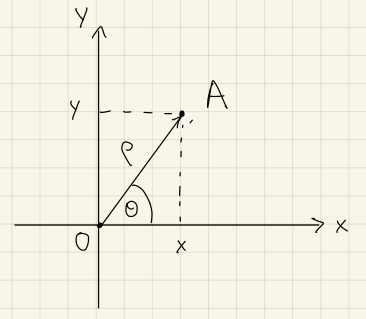
\includegraphics[width=0.40\textwidth]{coordinate-polari.png}}
     &
    \(A = (x,y) \in \R^2\) \hfill (coord.{ }cartesiane) \newline
    \(A = (\rho, \theta)\) \hfill (coord.{ }polari) \newline
    \hspace*{1cm}\(\downharpoonleft \ \downarrow \) \newline
    \hspace*{1cm}\(\downarrow \theta = \) angolo \newline
    \hspace*{1cm}\(\rho = \) lunghezza \newline
    \vspace{3mm} \newline
    \(\rho = \overline{OA} = d(A,\uzero) = \sqrt{x^{2}+y^{2}}\) \newline
    \(\theta = \arctan\left(\frac{y}{x}\right)\) \newline
\end{tabular}

\bigskip

Per passare da coordinare cartesiane a polari, basta usare la seguente relazione

\begin{equation*}
    \begin{cases}
        x - x_0 = \rho \cos\theta \\
        y - y_0 = \rho \sin\theta
    \end{cases}
    \ \implies
    \begin{cases}
        \rho = \sqrt{x^2 + y^2} \\
        \theta = \displaystyle \arctan\left(\frac{y}{x}\right) \pmod{2\pi}
    \end{cases} \\
\end{equation*}

\subsubsection{Limiti e coordinate polari}

\teorema{}{
    Sia \(f: D \subseteq \R^{2} \rightarrow \R \) e sia \(P_0=(x_0,y_0) \in D\) allora:

    \[
        \lim_{ (x,y) \to (x_0,y_0) } f(x,y) = l \ \iff \lim_{ \rho \to 0^{+} } f(x_0 + \rho\cos\theta ,\  y_0 + \rho\sin\theta ) = l
    \]

    \textbf{uniformemente rispetto a \(\theta \)}.
}

\defn{Uniformemente rispetto a \(\theta \)}{
    Dire che il limite è uniforme rispetto a \(\theta \) significa che il nostro limite (\(l\)) non dipende dalla scelta di \(\theta \), dove \(\theta \in (0,2\pi)\).
}

\defn{Limite finito con le coordinate polari}{
    Dire che

    \[
        \lim_{ \rho \to 0^{+} } f(x_0 + \rho\cos\theta ,\ y_0 + \rho\sin\theta ) = l
    \]

    significa quindi che:
    \medbreak{}

    \hspace*{5mm}
    \(\forall \varepsilon>0\),

    \hspace*{5mm}
    \(\exists \delta>0\) tale che \(\forall \rho \giventhat 0 < \rho < \delta\ ,  ~\forall \theta \in \lparen 0,2\pi \rbrack \)

    \hspace*{5mm}
    si ha: \(\big|f(x_0 + \rho\cos\theta ,\  y_0 + \rho\sin\theta  ) -l\big| < \varepsilon \)
}

Per dimostrare quanto abbiamo appena affermato, utilizzeremo il seguente procedimento che prende anche il nome di criterio del confronto.

\defn{Criterio del confronto}{
    Per far vedere che vale

    \[
        \lim_{ \rho \to 0^{+} } f(x_0 + \rho\cos\theta ,\ y_0 + \rho\sin\theta ) = l
    \]

    è sufficiente mostrare che esiste una funzione strettamente positiva \(g\) che dipende solo da \(\rho \), quindi \(\exists g(\rho) > 0\), tale che:

    \[
        0 \le \big|f(x_0 + \rho\cos\theta ,\  y_0 + \rho\sin\theta  ) -l\big| \le  g(\rho)
    \]

    dove si ha che:
    \[
        \lim_{\rho \to 0^+} g(\rho) \rightarrow 0
    \]

    Se accade che il limite dipende da \(\theta \), allora il limite non esiste.
}

\pagebreak

\subsubsection{Esempi ed esercizi}

\subsubsection*{Esempio precedente rifatto con le coordinate polari}

Avevamo già mostrato che il limite non esiste:

\[
    \lim_{ (x,y) \to (0,0) } \frac{xy}{x^{2}+y^{2}}
\]

\begin{equation*}
    \begin{cases}
        x = \rho\cos\theta \\
        y = \rho\sin\theta
    \end{cases}
\end{equation*}

il limite diventa:

\[
    \lim_{ \rho \to 0^{+} } \frac{\rho\cos\theta \cdot\rho\sin\theta }{\rho^{2}\cos^{2}\theta  + \rho^{2}\sin^{2}\theta } = \lim_{ \rho \to 0^{+} } \frac{\rho^{2}\cos\theta \sin\theta }{\rho^{2} \cdot (1)} = \frac{1}{2}\sin(2\theta)
\]

\(\implies \) limite dipende dalla scelta di \(\theta \).

\(\implies \) il limite non esiste dato che non è uniforme rispetto a \(\theta \)

\filbreak{}
\subsubsection*{Altro esempio}

Calcolare, se esiste, il seguente limite:

\[
    \lim_{ (x,y) \to (0,0) } \frac{xy}{\sqrt{x^{2}+y^{2}}}
\]

Trasformiamo in coordinate polari:

\[
    \lim_{ \rho \to 0^{+} } \frac{\rho\cos\theta \rho\sin\theta }{\sqrt{\rho^{2}}} = \lim_{ \rho \to 0^{+} } \frac{\rho^{2}\cos\theta \sin\theta }{\rho} = \lim_{ \rho \to 0^{+} } \rho\cos\theta\sin\theta = 0
\]

Dimostriamo che il candidato a essere limite, \(l=0\), esiste usando il criterio del confronto. Troviamo una \(g(\rho)\):

\[
    \rho\cos\theta\sin\theta = \rho\frac{\sin(2\theta)}{2} \le \left|\rho\frac{\sin(2\theta)}{2}\right| = \rho\left|\frac{\sin(2\theta)}{2}\right| \le \rho{\frac{1}{2}} = g(\rho)
\]

Questa \(g(\rho)\) dipende solo da \(\rho \) e \(\lim_{\rho \to 0^+} g(\rho) = 0\), quindi ok. Possiamo dunque dire che il limite esiste:

\[
    0 \le \left| \rho\cos\theta \sin\theta  -0 \right| \le \frac{1}{2}\rho
\]

\filbreak{}
\subsubsection*{Esercizio 1}

Calcolare, se esiste, il seguente limite:

\[
    \lim_{ (x,y) \to (0,0) } \frac{\arctan\left({(x+y)}^{2}\right)}{x^{2}}
\]

ricordo che \(\arctan(x) \sim x \text{ per } x\to0\);

consideriamo la funzione lungo l'asse x quindi con \(y=0\):

\[
    \lim_{ \begin{smallmatrix}(x,y) \to (0,0) \\ y=0\end{smallmatrix} } \frac{\arctan\left({(x+y)}^{2}\right)}{x^{2}}= \underbrace{\lim_{ x \to 0 } \frac{\arctan\left(x^{2}\right) }{x^{2}}}_{\text{limite notevole}} = 1
\]

vedo per la bisettrice (\(y=x\)):

\[
    \lim_{ \begin{smallmatrix}(x,y) \to (0,0) \\ y=x\end{smallmatrix} } \frac{\arctan\left({(x+y)}^{2}\right)}{x^{2}} = \lim_{ x \to 0 } \frac{\arctan\left({(x+x)}^{2}\right)}{x^{2}} = \lim_{ x \to 0 } \frac{\arctan\left({4x}^{2}\right)}{x^{2}} = 4
\]

quindi il limite non esiste.

\filbreak{}
\subsubsection*{Esercizio 2}

Calcolare, se esiste, il seguente limite:

\[
    \lim_{ (x,y) \to (0,0) } \frac{{(x+y)}^{2}}{x^{2}+y^{2}}
\]

vediamo cosa succede lungo l'asse x (\(y=0\)):

\[
    \lim_{ (x,y) \to (0,0) } \frac{{(x+y)}^{2}}{x^{2}+y^{2}} = \lim_{ x \to 0 } \frac{x^{2}}{x^{2}} = 1
\]

per \(y=x\):

\[
    \lim_{ (x,y) \to (0,0) } \frac{{(x+y)}^{2}}{x^{2}+y^{2}} = \lim_{ x \to 0 } \frac{{(x+x)}^{2}}{x^{2}+x^{2}} = 2
\]

quindi il limite non esiste.

\filbreak{}
\subsubsection*{Esercizio 3 {-} Definizione di continuità}

Calcolare, se esiste, il seguente limite:

\[
    \lim_{ (x,y) \to (0,0) } \frac{x^{2}-y^{2}}{x^{2}+y^{2}+5}
\]

Essendo questo un limite di funzioni continue (polinomi in due variabili), applicando la definizione di continuità posso dire che il limite è la funzione valutata nel punto di accumulazione.

Quindi il limite è \(= f(0,0) = 0\).

\filbreak{}
\subsubsection*{Esercizio 4 {-} Coordinate polari}

Calcolare, se esiste, il seguente limite:

\[
    \lim_{ (x,y) \to (0,0) } \frac{x\ln(1+x^{3})}{y(x^{2}+y^{2})}
\]

ricordo che \(\ln(1 + x) \sim x \text{ per } x\to0\);

passiamo in coordinate polari e dunque il limite diventa:

\begin{align*}
    \lim_{ \rho \to 0^{+} } \frac{\rho\cos\theta \cdot\ln\left(1+\rho^{3}\cos^{3}\theta \right)}{\rho\sin\theta \cdot\left(\rho^{2}\cos^{2}\theta  + \rho^{2}\sin^{2}\theta \right)} & = \lim_{ \rho \to 0^{+} } \frac{\rho\cos\theta \cdot\ln(1+\rho^{3}\cos^{3}\theta )}{\rho\sin\theta \cdot (\rho^{2}) }  \\
                                                                                                                                                                                     & = \lim_{ \rho \to 0^{+} } \frac{\rho\cos\theta \cdot \rho^{3}\cos^{3}\theta}{\rho^{3}\sin\theta }                      \\
                                                                                                                                                                                     & = \lim_{ \rho \to 0^{+} } \frac{\rho^{4}\cos^{4}\theta }{\rho^{3}\sin\theta } = \lim_{ \rho \to 0^{+} } \rho M(\theta)
\end{align*}

dove \(M(\theta) = \frac{\cos^{4}\theta }{\sin\theta }\) si nota che per ogni \(\theta \neq \pm \pi \) il limite è zero.

A questo punto non possiamo concludere subito che il limite non esiste, perché il denominatore non è sempre \(\ne 0\). Bisogna quindi analizzare, attraverso il teorema del confronto, il comportamento della funzione quando il denominatore è \(= 0\).

Ovvero, considerato il candidato a essere limite, 0, controlliamo se nei punti in cui la funzione non è definita il limite è uguale o meno.

\[
    \underset{\theta}{\sup} \bigl|\rho M(\theta)\bigr| = \sup\left|\rho \frac{\cos^{4}\theta }{\sin\theta }\right|
\]

se la nostra funzione, su \(\theta \in (0,2\pi)\) fosse finita, allora:

\[
    |M(\theta) | \le \bar{e}
\]

il \(\sup \) cioè è finito, e sono quindi a posto; ma \(M(\theta) \) non è limitata. Ad esempio, in \(\theta= \pi \) abbiamo un asintoto verticale:

\[
    \lim_{ \theta \to \pi } \frac{\cos^{4}\theta }{\sin\theta }= +\infty
\]

allora per studiare il limite vediamo che succede muovendoci verso l'origine lungo curve che sono tangenti all'asse x. Ovvero, curve (funzioni) la cui retta tangente in \((0,0)\) forma un angolo \(\theta = \pi \) con l'asse \(x\).

Consideriamo quindi \(y=x^{2}\):

\begin{align*}
    f(x,x^{2}) & = \frac{x\ln(1+x^{3})}{x^{2}(x^{2}+x^{4})} = \frac{\ln(1+x^{3})}{x^{3}(1+x^{2})} \overset{\text{per limite notevole}}{=} \frac{\cancel{x^3}}{\cancel{x^{3}}(1+x^{2})} \quad \xrightarrow[x \to 0]{}\  1 \implies \text{limite } \nexists
\end{align*}

\filbreak{}
\subsubsection*{Esercizio 5 {-} Limite con parametro reale}

Studiare l'esistenza del limite al variare del parametro reale \(\alpha \in \R \), con \(\alpha >0\):

\[
    \lim_{ (x,y) \to (1,0) } \frac{(x^2-2x+1)y}{{(x^2-2x+1+y^2)}^{\alpha}} =
    \lim_{ (x,y) \to (1,0) } \frac{{(x-1)}^2 y}{{\left({(x-1)}^2 + y^2\right)}^{\alpha}}
\]

Noto che questa funzione è definita su tutto \(\R \), e passo in coordinate polari:

\begin{equation*}
    \begin{cases}
        x = 1+\rho\cos\theta \\
        y = 0+\rho\sin\theta
    \end{cases}
\end{equation*}

allora:

\begin{align*}
    \lim_{ \rho \to 0^{+} } \frac{{(1 + \rho\cos\theta  -1 )}^{2} \rho\sin\theta }{{\left({(1+\rho\cos\theta  -1)}^{2}+\rho^{2}\sin^{2}\theta \right)}^{\alpha}} & = \lim_{ \rho \to 0^{+} } \frac{\rho^{2}\cos^{2}\theta \rho\sin\theta }{{\left(\rho^{2}\cos^{2}\theta +\rho^{2}\sin^{2}\theta \right)}^{\alpha}} \\
                                                                                                                                                                 & = \lim_{ \rho \to 0^{+} } \frac{\rho^{3}\cos^{2}\theta \sin\theta }{\rho^{2\alpha} \cdot 1}                                                      \\
                                                                                                                                                                 & = \lim_{ \rho \to 0^{+} } \rho^{3-2\alpha} \cos^{2}\theta \sin\theta
\end{align*}

Dato che \(\rho^x \xrightarrow[\rho \to 0^+]{} 0\) se \(x > 0\), analizziamo i vari casi ricordando che \(\alpha > 0\) per le condizioni iniziali:

\begin{itemize}
    \item Se \(3-2\alpha > 0\) ovvero \(\bm{0<\alpha < \frac{3}{2}}\):

          poiché \(\left\vert \cos^{2}\theta \sin\theta \right\vert \le 1\), attraverso il confronto diretto possiamo dire che:

          \[
              0 \le \left\vert\rho^{3-2\alpha}\cos^{2}\theta \sin\theta\right\vert = \rho^{3-2\alpha}\left\vert\cos^{2}\theta \sin\theta\right\vert \le \rho^{3-2\alpha} \to 0
          \]
          \(\implies \) il limite vale 0
    \item Se \(\bm{\alpha = \frac{3}{2}}\):

          \[
              \implies \lim_{\rho \to 0^+} \cancel{\rho^0} \cos^{2}\theta \sin\theta = \cos^{2}\theta \sin\theta
          \]

          dipende da \(\theta \) quindi il limite non esiste.
    \item Se \(\bm{\alpha > \frac{3}{2}}\):

          \[
              \alpha > \frac{3}{2} \implies \rho^{3-2\alpha} = \frac{1}{\rho^{2\alpha-3}}
          \]
          \[
              \implies \lim_{ \rho \to 0^{+} } \rho^{3-2\alpha} \cos^{2}\theta \sin\theta = \lim_{ \rho \to 0^{+} } \frac{\cos^{2}\theta \sin\theta}{\rho^{2\alpha-3}} = \pm \infty \ \text{ a seconda di } \theta
          \]

          Quindi il limite non esiste anche in questo caso. Da notare che se \(\sin\theta \) o \(\cos\theta \) fossero \(=0\), sarebbe più complesso, ma il limite comunque non esisterebbe.

\end{itemize}

\filbreak{}
\subsubsection*{Esercizio 6 {-} Studio di continuità}

Studiamo la continuità della seguente funzione nel suo dominio di definizione:

\[
    f(x,y)=
    \begin{cases}
        2x+3y+10 & \text{se}\ {(x-1)}^{2}+{(y-3)}^{2} \ge 4 \\
        x+4y+10  & \text{se}\ {(x-1)}^{2}+{(y-3)}^{2} < 4
    \end{cases}
\]

Abbiamo due piani, e una circonferenza. Devo vedere cosa succede a:
\[
    \lim_{ (x,y) \to (x_0,y_0) } x+4y+10 \qquad \forall (x_0,y_0) \in \{(x,y) \in \R^2 \giventhat {(x-1)}^{2}+{(y-3)}^{2} = 4\}
\]
Analizziamo l'intersezione tra questi due piani e la circonferenza:

\begin{equation*}
    \begin{cases}
        2x+3y+10 = x +4y +10 \\
        {(x-1)}^{2} + {(y-3)}^{2} = 4
    \end{cases}
\end{equation*}

verifichiamo se il sistema ha soluzione:
\begin{align*}
     & \begin{cases}
           x-y=0 \\
           {(x-1)}^{2} + {(y-3)}^{2} = 4
       \end{cases}\implies
    \begin{cases}
        x=y \\
        y^{2}-2y+1+y^{2}-6y+9=4
    \end{cases} \implies
    \begin{cases}
        x=y \\
        2y^{2}-8y + 6 = 0
    \end{cases}                 \\ \\
     & \implies \begin{cases}
                    x=y \\
                    y^{2}-4y+3=0
                \end{cases} \implies
    \begin{cases}
        x=y \\
        (y-3)(y-1) = 0
    \end{cases} \implies
    (x,y) \in \{(1,1), (3,3)\}
\end{align*}

Quindi possiamo concludere che la funzione \(f(x,y)\) è continua nei punti \((1,1)\) e \((3,3)\) ma non è continua su tutto \(\R^2\). Questo in quanto i due piani si intersecano solo in quei due punti, e non lungo tutta la circonferenza \({(x-1)}^{2}+{(y-3)}^{2} = 4\). Basta quindi prendere un qualsiasi altro punto sulla circonferenza, diverso da quei due, che il limite di \(x+4y+10\) in quel punto sarà diverso dalla funzione valutata nello stesso punto (dato che i piani non si intersecano).

\begin{center}
    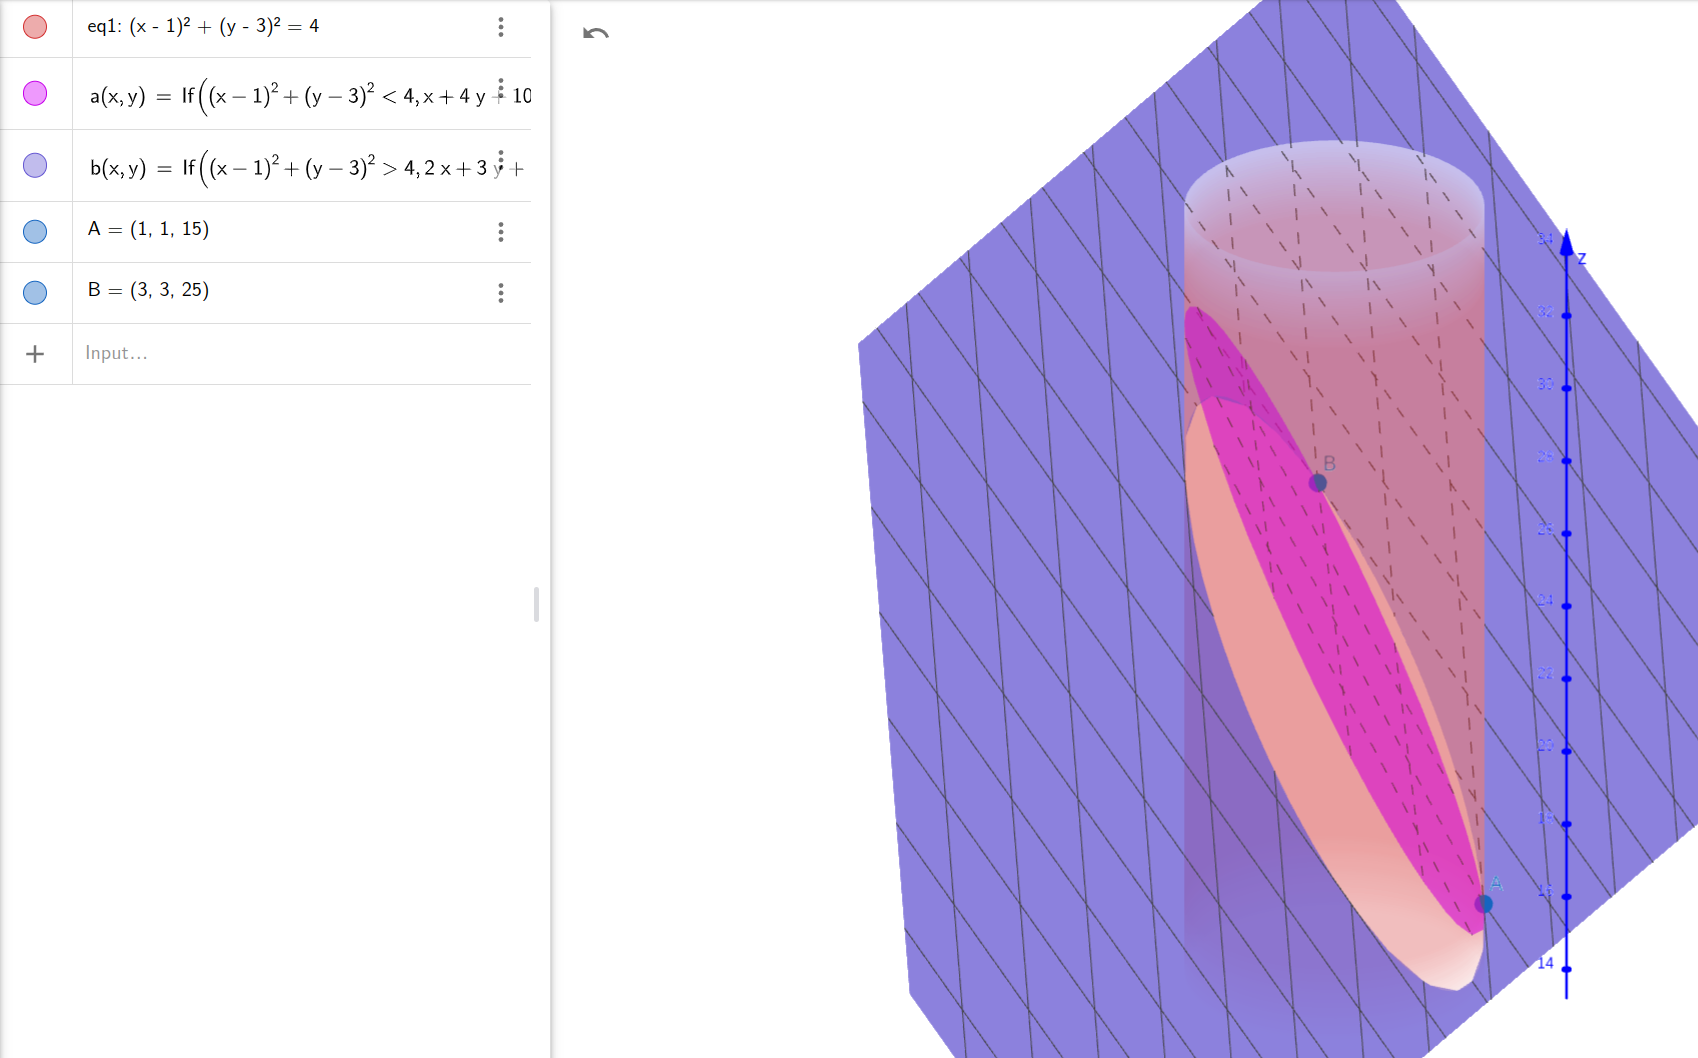
\includegraphics[width=0.85\textwidth]{limiti-esercizio-6.png}
\end{center}

\filbreak{}
\subsubsection*{Esercizio 7 {-} Studio di continuità}

Studiamo la continuità della seguente funzione, \(f: \R^2 \to \R \), nel suo dominio di definizione:

\[
    f(x,y) = \begin{cases*}
        0                                                                      & se \((x,y) = (1,1)\)   \\
        \displaystyle{\frac{e^{(x-1)+(y-1)} -1}{\sqrt{{(x-1)}^2 + {(y-1)}^2}}} & se \((x,y) \ne (1,1)\)
    \end{cases*}
\]

Affinché \(f(x,y)\) sia continua su tutto \(\R^2\) devo mostrare che

\[
    \lim_{(x,y) \to (1,1)} f(x,y) = \lim_{(x,y) \to (1,1)} \frac{e^{(x-1)+(y-1)} -1}{\sqrt{{(x-1)}^2 + {(y-1)}^2}} = f(1,1) = 0
\]

Guardiamo cosa fa la funzione lungo \(x=1\):

\[
    \lim_{\begin{smallmatrix}(x,y) \to (1,1) \\ x=1\end{smallmatrix}} f(x,y) =
    \lim_{y \to 1} \frac{e^{(y-1)} -1}{\sqrt{{(y-1)}^2}} =
    \lim_{y \to 1} \frac{e^{(y-1)} -1}{|y-1|} =
    \left[\frac{0}{0}\right] =
    \lim_{y \to 1} \frac{e^{(y-1)}}{\pm 1} = \pm 1
\]

Quindi il limite \(\nexists \)

Questo esercizio si poteva risolvere anche utilizzando le coordinate polari e facendo vedere che il limite non è uniforme rispetto a \(\theta \). Infatti, svolgendo i passaggi, il limite viene \(= \cos\theta + \sin\theta \)

\newpage
\subsection{Rappresentazioni di funzioni}

\subsubsection{Funzioni in \texorpdfstring{\(\R^2\)}{R2}}

Consideriamo una funzione \(f: D \subseteq \R^2 \to \R \) che associa \((x,y) \mapsto f(x,y)\).

L'insieme \(D\) è il dominio della funzione, ovvero, l'insieme dei punti \((x,y) \in \R^2\) per cui \(f(x,y) \in \R \)

\[D = \{(x,y) \in \R^2 \giventhat f(x,y) \in \R \} \subseteq \R^2 \]

Definiamo tutti i valori che può assumere la funzione con l'immagine della funzione che è definita come segue:

\[\im{f} = \{z \in \R \giventhat z = f(x,y), ~\forall (x,y) \in D\} \subset \R \]

\subsubsection*{Esempi}

\begin{enumerate}
    \item \(f(x,y) = 3x + 2y + 5 \implies D=\R^2\)
    \item \(f(x,y) = \frac{\ln(x+y)}{x-3}\)
          \begin{align*}
              D & = \{(x,y) \in \R^2 \giventhat x-3 \ne 0;\ x+y > 0\} & \text{(\(x+y > 0 \to \) disequazione in \(\R^2\))} \\
                & = \{(x,y) \in \R^2 \giventhat x \ne 3;\ y > -x\}
          \end{align*}

          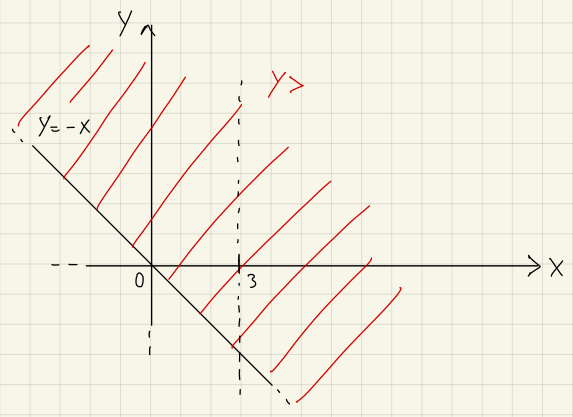
\includegraphics[width=0.5\textwidth]{grafico-di-funzioni-2.png}
\end{enumerate}

\filbreak{}
\subsubsection{Insiemi del piano \texorpdfstring{\(\R^2\)}{R2} determinati da disequazioni}

Consideriamo il caso reale. Sia \(f: I \subset \R \to \R \) continua, definiamo il suo grafico:

\[\graf{f} = \{(x,y) \in \R^2 \giventhat y=f(x),\ x \in I \} = \underbrace{\{(x,f(x))\}}_{\text{con \(x \in I\)}}\]

Possiamo quindi definire il concetto di sopragrafico e sottografico di una funzione:

\defn{Sopragrafico}{
    Si definisce sopragrafico la parte di piano tale che:

    \[y \ge f(x) \implies \{(x,y) \in \R^2 \giventhat x \in I;\ y \ge f(x) \} \]

    Oppure, nella forma in senso stretto:

    \[y > f(x) \implies \{(x,y) \in \R^2 \giventhat x \in I;\ y > f(x) \} \]
}

\defn{Sottografico}{
    Si definisce sottografico la parte di piano tale che:

    \[y \le f(x) \implies \{(x,y) \in \R^2 \giventhat x \in I;\ y \le f(x) \} \]

    Oppure, nella forma in senso stretto:

    \[y < f(x) \implies \{(x,y) \in \R^2 \giventhat x \in I;\ y < f(x) \} \]
}

Ad esempio, data una qualche \(f(x)\) su un intervallo \(I=[a,b]\), abbiamo in rosso il rispettivo sopragrafico, e in blu il rispettivo sottografico:

\medskip
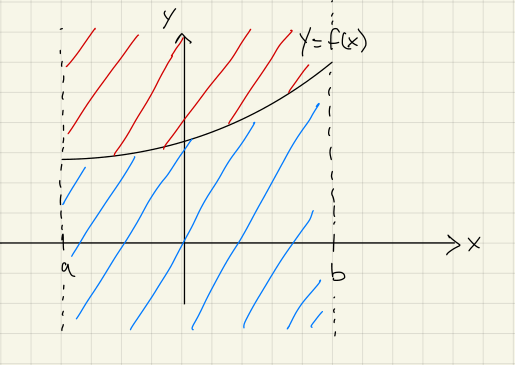
\includegraphics[width=0.45\textwidth]{grafico-di-funzioni-sopra-sotto.png}

\filbreak{}

\subsubsection*{Esempi}

\begin{enumerate}
    \item \(y \ge \ln(x)\) con \(0<x<2\)

          \medskip
          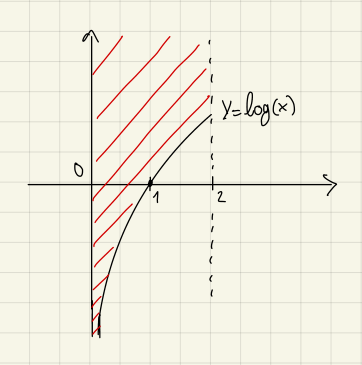
\includegraphics[width=0.4\textwidth]{grafico-di-funzioni-3.png}

    \item \(2x - 3y +1 \ge 0\)

          \(y \le \frac{2}{3}x + \frac{1}{3}\)

          \medskip
          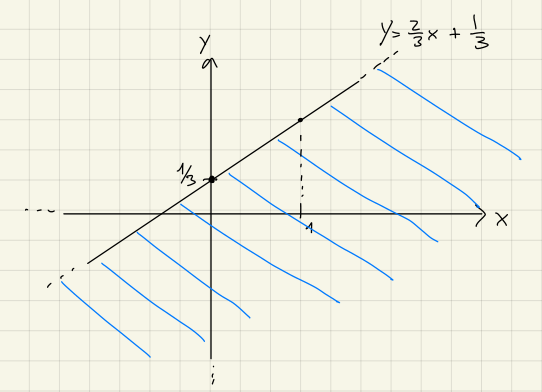
\includegraphics[width=0.5\textwidth]{grafico-di-funzioni-4.png}
\end{enumerate}

\filbreak{}
\subsubsection{Generalizzazione teorema degli zeri}

Vediamo come applicare il teorema degli zeri visto in \(\R \) per funzioni in \(\R^2\) attraverso un esempio.

Sia \(f(x,y) = x^2 - y^2 -1\) la nostra funzione. Vogliamo studiarne il segno e quindi vogliamo capire dove \(x^2-y^2 -1 \ge 0\). Iniziamo disegnando il grafico di quando \(f(x,y) = 0\), ovvero dell'iperbole:

\begin{center}
    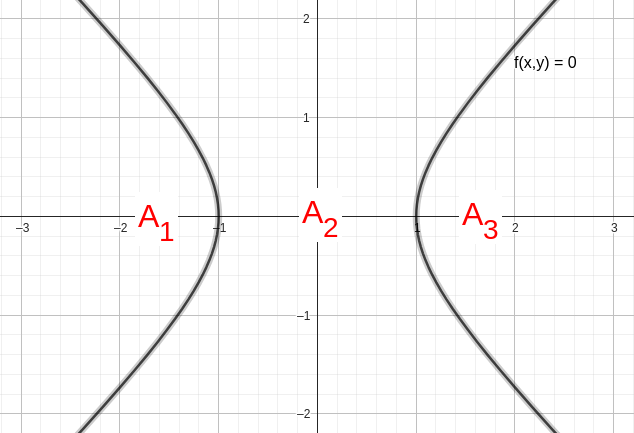
\includegraphics[width=0.5\textwidth]{teorema-degli-zeri-1.png}
\end{center}

Il grafico divide il piano nell zone \(A_1, A_2, A_3\) che sono insiemi aperti e connessi dove \(f(x,y) \ne 0\).

Con queste condizioni in ognuna delle zone il segno della funzione \underline{non} cambia.

(\textit{Generalizzazione teorema degli zeri})

Nel nostro caso \(f(x,y)\) è continua in \(\R^2\)

\(f(x,y)\) definisce un aperto del piano dato da un certo numero di aperti. Supponiamo che tali aperti siano in numero finito \(A_1, A_2, \ldots, A_n\)

Studio il segno di \(f(x,y)\) in ognuno di questi insiemi \(\underset{i=1, \ldots, n}{A_i}\).

In \(A_1\): \(f(x,y) \ne 0\) e dunque o \(f(x,y) > 0\) o \(f(x,y) < 0\). Essendo \(A_1\) aperto e connesso si ha che il segno di \(f(x,y)\), che è continua in \(A\), non cambia. Infatti, se esistessero due punti distinti di \(A_1\) in cui \(f(x,y)\) ha segno opposto, allora ci deve essere un punto in \(A_1\) in cui \(f(x,y) = 0\), ma \(f(x,y) \ne 0 ~\forall (x,y) \in A\).

In \(A_2, A_3\) si applica lo stesso ragionamento.

Studio quindi il segno in un punto comodo per ogni regione:

\begin{itemize}
    \item In \(A_1\): \(f(-2,0) = {(-2)}^2 + 0^2 - 1 = 3 > 0\)

          Dunque, \(f(x,y) > 0\) in \(A_1\) \((\forall (x,y) \in A_1)\)
    \item In \(A_2\): \(f(0,0) = 0^2 + 0^2 - 1 = -1 < 0\)

          Dunque, \(f(x,y) < 0\) in \(A_2\) \((\forall (x,y) \in A_2)\)
    \item In \(A_3\): \(f(2,0) = 2^2 + 0^2 - 1 = 3 > 0\)

          Dunque, \(f(x,y) > 0\) in \(A_3\) \((\forall (x,y) \in A_3)\)
\end{itemize}

Possiamo quindi aggiornare il grafico iniziale colorando le zone \(A_1\) e \(A_3\) dove \(f(x,y) > 0\).

\subsubsection*{Esempio}

Determinare l'insieme di definizione \(D \subset \R^2\) della seguente funzione, \(f: D \subseteq \R^2 \to \R \):

\[f(x,y) = \frac{\ln(x^3 - y)}{\sqrt{1-xy}}\]

Procediamo trovando il dominio della funzione:

\begin{align*}
    D & = \{(x,y) \in \R^2 \giventhat f(x,y) \in \R \}                      \\
      & = \{(x,y) \in \R^2 \giventhat (1-xy > 0) \text{ e } (x^3 -y > 0) \} \\
      & = \{(x,y) \in \R^2 \giventhat (xy < 1) \text{ e } (y < x^3) \}      \\
\end{align*}

Graficamente, è la parte di piano colorata in viola della seguente immagine:

\begin{center}
    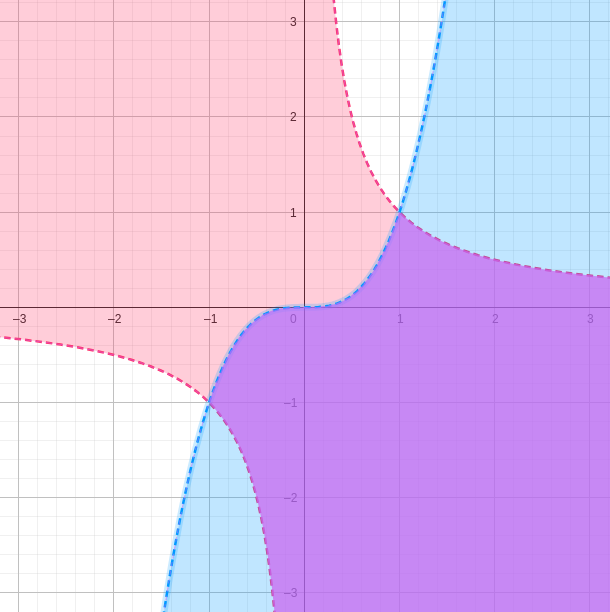
\includegraphics[width=0.6\textwidth]{esercizio-dominio-funzione-1.png}
\end{center}

\newpage
\subsubsection{Grafico di funzioni a due variabili}

Sia \(f: D \subseteq \R^2 \to \R \);

Il grafico di \(f(x,y)\) è un sottoinsieme \(S \subset \R^3 \).

\[\graf{f} = \{(x,y,z) \in \R^3 \giventhat z = f(x,y) \text{ con } (x,y) \in D\} \subset \R^3\]

\begin{center}
    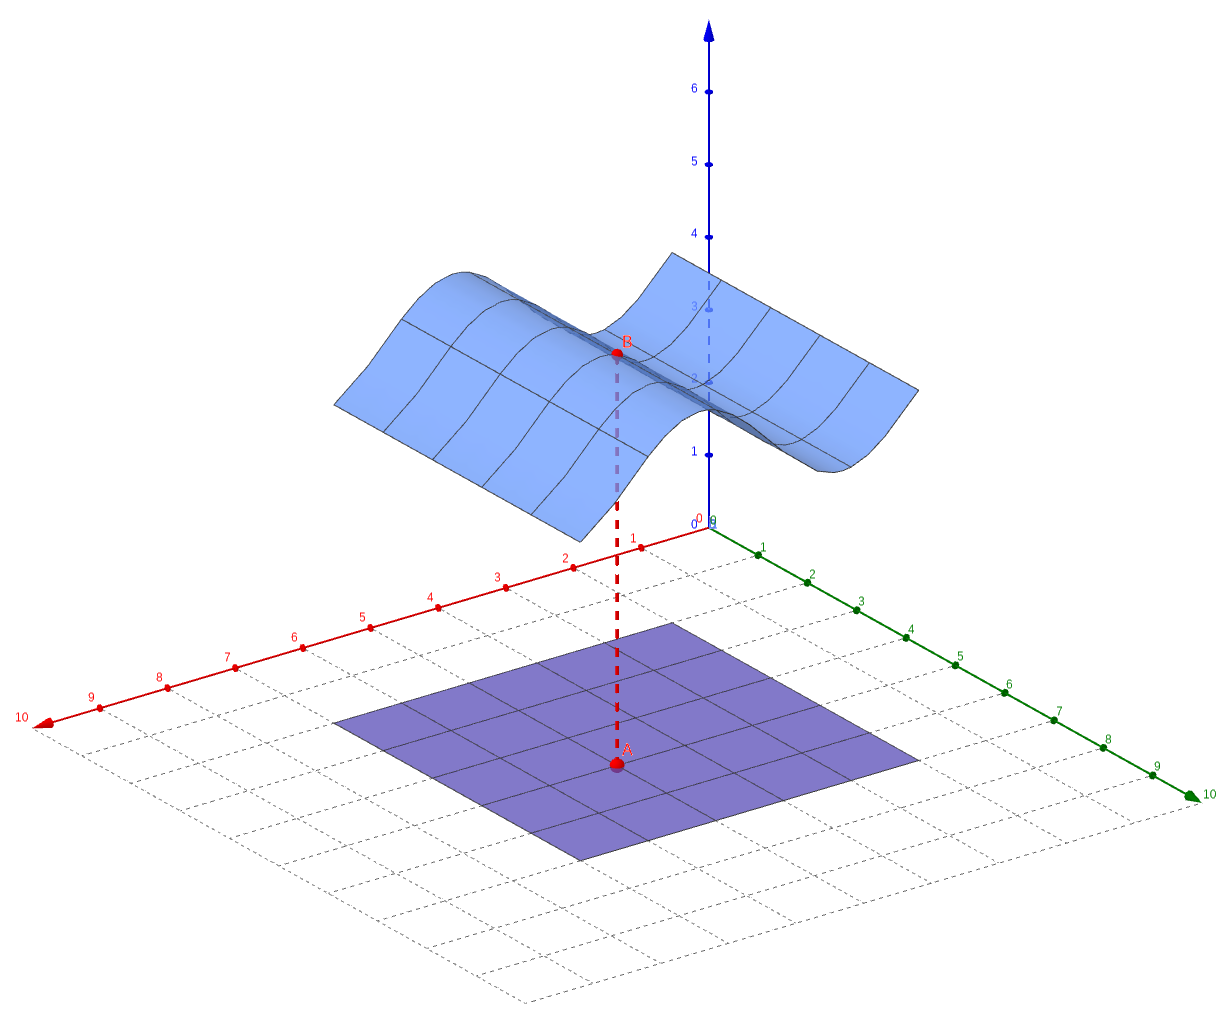
\includegraphics[width=0.8\textwidth]{grafico-di-funzione-2-variabili.png}
\end{center}

\begin{itemize}
    \item La nostra funzione \(f(x,y)\) è rappresentata con il colore celeste;
    \item La proiezione di \(S\) su \((x,y)\) è rappresentata con il colore viola;
    \item Dato un punto \((x,y,0) = A\), abbiamo il rispettivo punto \(B = (x,y,f(x,y))\)
    \item La distanza tra \(A\) e \(B\), rappresentata dal segmento tratteggiato, è chiamata ``Quota''.
\end{itemize}

Per studiare quindi il grafico di una funzione a 2 variabili, affetto il grafico con dei piani e studio le sezioni ottenute.

Le sezioni \underline{trasversali} intersecano \(S\) con i piani:
\begin{itemize}
    \item \(x=k\)
    \item \(y=k\)
    \item \(z=k \rightarrow \) piano orizzontale; otteniamo una sezione sul piano \((x,y)\)
\end{itemize}

Queste sono chiamate \textbf{Tracce} della funzione e si definiscono come segue:

\[
    S \subset \R^3\
    \begin{cases}
        \graf{f} \\
        x=k
    \end{cases}
    \implies
    \begin{cases}
        z = f(x,y) \\
        x=k
    \end{cases}
    \implies
    z = f(k,y) \quad \text{grafico nel piano }(y,z)
\]
\[
    S \subset \R^3\
    \begin{cases}
        \graf{f} \\
        y=k
    \end{cases}
    \implies
    \begin{cases}
        z = f(x,y) \\
        y=k
    \end{cases}
    \implies
    z = f(x,k) \quad \text{grafico nel piano }(x,z)
\]
\[
    S \subset \R^3\
    \begin{cases}
        \graf{f} \\
        z=k
    \end{cases}
    \implies
    \begin{cases}
        z = f(x,y) \\
        z=k
    \end{cases}
    \implies
    k = f(k,y) \quad \text{grafico nel piano }(x,y)
\]

Le intersezioni del grafico con i piani \(z=k\) sono chiamate \textbf{insiemi di livello K} della funzione.

Queste sono anche chiamate \textbf{curve di livello} se relative a ``curve'', ovvero se la funzione non è costante. Queste sono le proiezioni sul piano \(xy\) delle curve ottenute dall'intersezione del grafico \(f(x,y)\) con il piano \(z=k\).

Vediamo un esempio della curva di livello della funzione \(z=x+y\) che corrisponde al livello \(z=2\):

\begin{center}
    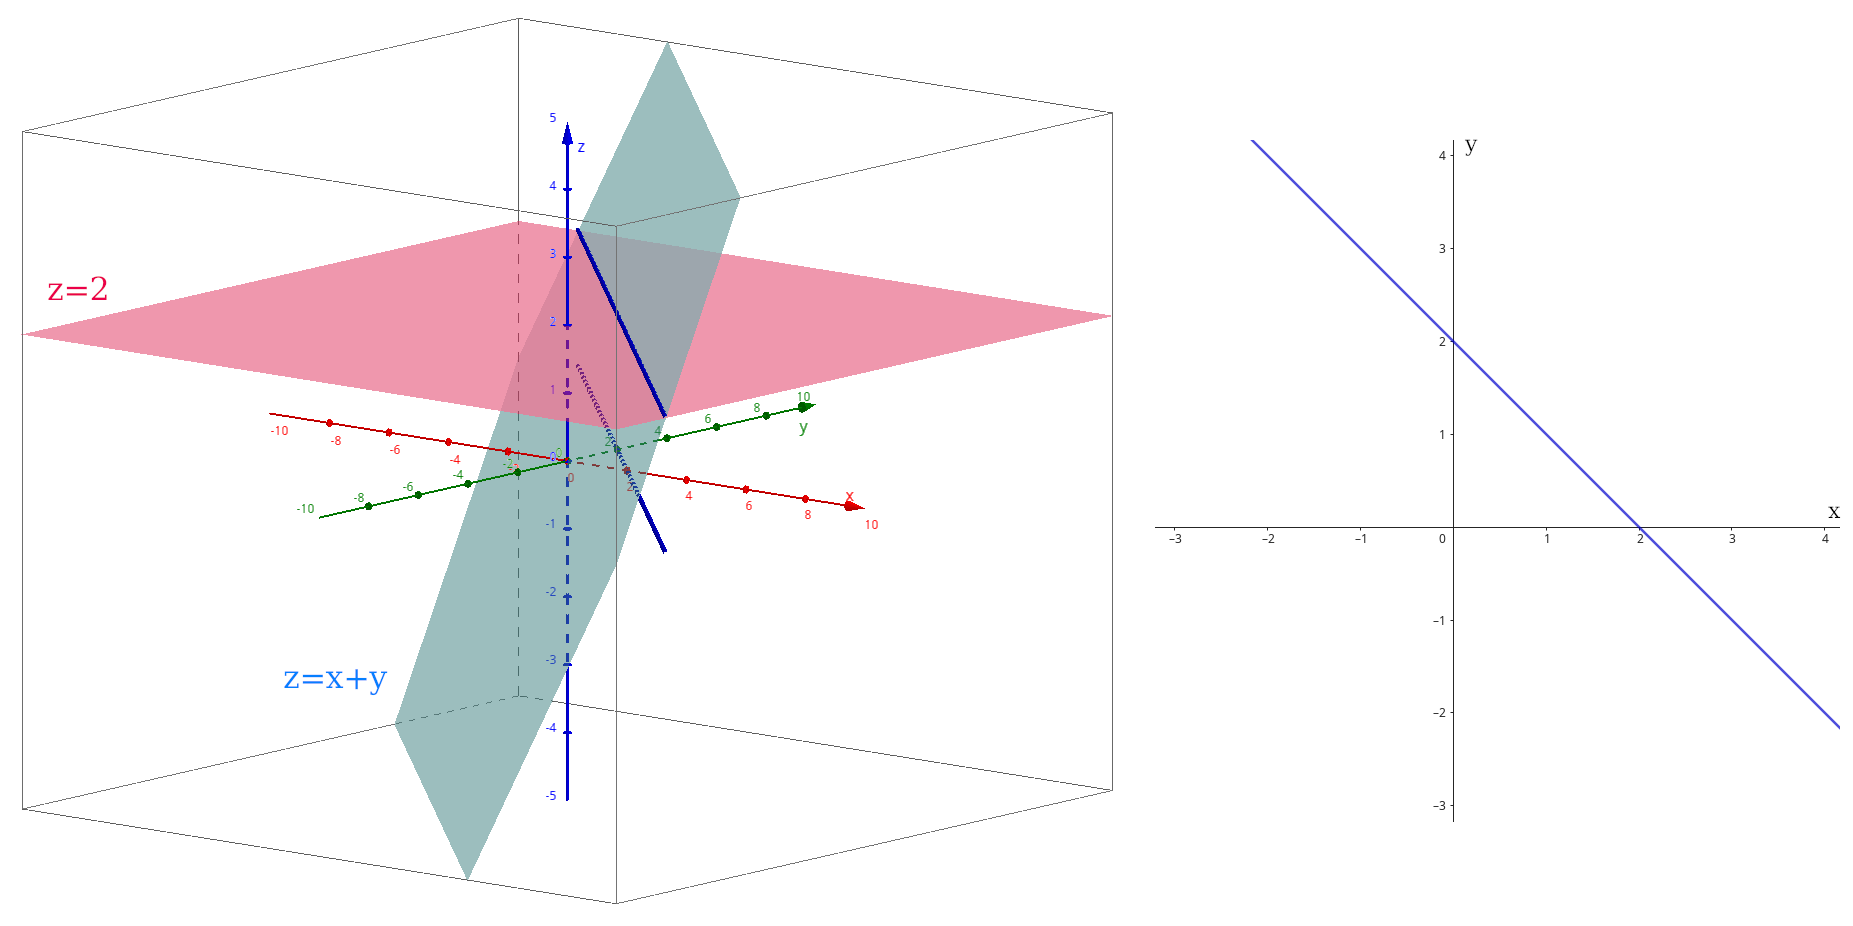
\includegraphics[width=\textwidth]{curve-di-livello-esempio-3.png}
\end{center}

A sinistra abbiamo i due piani che si intersecano, mentre a destra abbiamo la curva di livello rappresentata sul piano \(xy\).

\pagebreak
\subsubsection{Insiemi o curve di livello}

Come abbiamo appena visto, le \textbf{curve di livello} sono le intersezioni del grafico con il piano \(z=k\).

Vediamo la questione in pratica; prendiamo la funzione, \(f: \R^2 \to \R \), definita da:
\[
    f(x,y) = x^2 + y^2
\]
L'insieme delle curve di livello si scrive:

\[
    E_k = \left\{ (x,y) \in \R^{2} \giventhat x^{2}+y^{2}=k \right\}
\]

Se consideriamo i punti \((x,y)\) che stanno nell'insieme di livello \(k=1\) della funzione, questi sono i punti che stanno sulla circonferenza di centro \((0,0)\) di raggio 1:

\[
    E_1 = \left\{ (x,y) \in \R^{2} \giventhat x^{2}+y^{2}=1 \right\}
\]

\begin{center}
    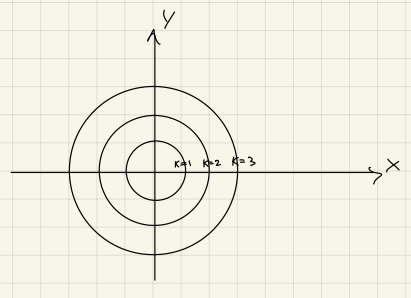
\includegraphics[width=0.5\textwidth]{curve-di-livello-esempio.png}
\end{center}

\filbreak{}
Quindi il grafico di \(f\) ha la seguente forma:

\begin{center}
    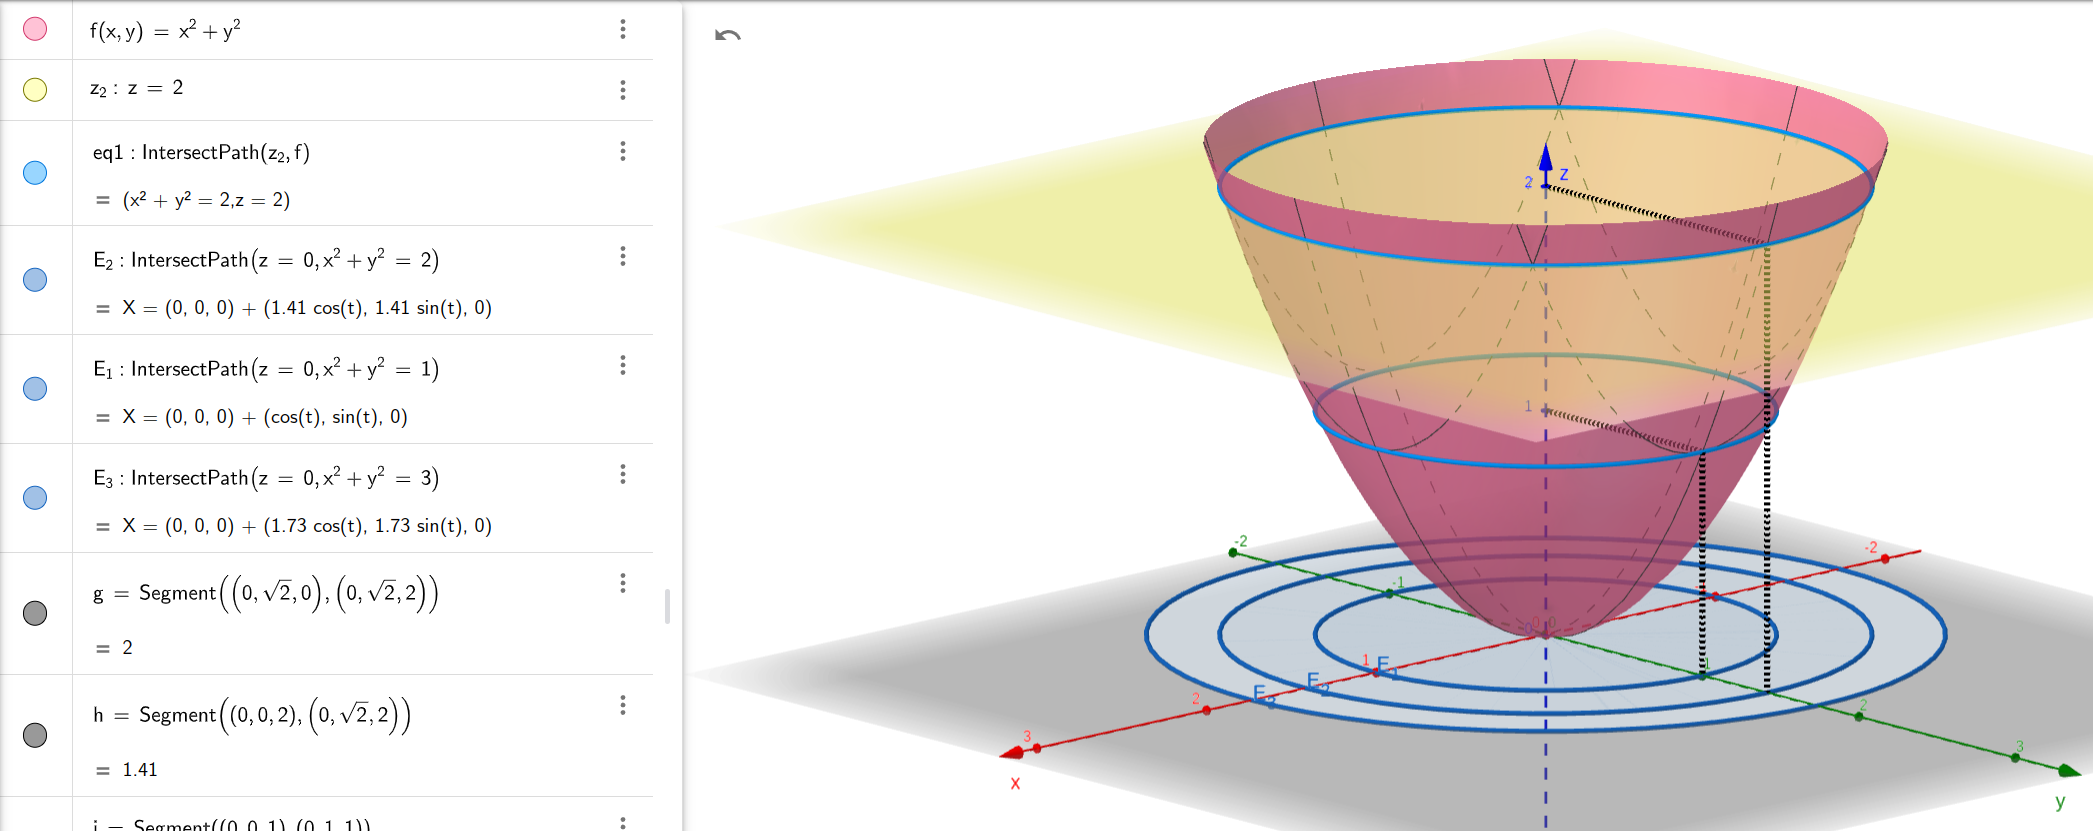
\includegraphics[width=\textwidth]{curve-di-livello-esempio-2.png}
\end{center}

\pagebreak
\subsubsection{Esempi {-} Domini}

\subsubsection*{Esempio 1}

Determinare l'insieme di definizione della seguente funzione:

\[
    z = \sqrt{1-x^{2}-y^{2}}
\]

\(D = \{(x,y) \in \R^2 \giventhat f(x,y) \in \R \} = \{(x,y) \in \R^{2} \giventhat x^{2}+y^{2} \le 1\} \)

Questo vuol dire che la funzione è definita all'interno della circonferenza di funzione:
\[
    f(x,y) = x^2+y^2-1
\]

Essendo questa una circonferenza di raggio 1 con centro l'origine degli assi, possiamo dire che il dominio \(D\) costituito dai punti interni a questa circonferenza è chiuso.

Inoltre, possiamo analizzare le curve di livello:
\[
    E_k = \{(x,y) \in D \giventhat x^2+y^2=1+k\}
\]
Quindi:
\begin{itemize}
    \item \(k<-1 \implies E_k = \emptyset \)
    \item \(-1\le k \le 0 \implies E_k = \{(x,y)\in \R^{2} \giventhat x^2+y^2=1+k\} \)
    \item \(k>0 \implies E_k = \emptyset \)
\end{itemize}

\filbreak{}
\subsubsection*{Esempio 2}

Determinare l'insieme di definizione della seguente funzione:

\[
    z = \sqrt{1-x^{2}}+\sqrt{1-y^{2}}
\]

devo imporre il dominio:

\[
    \{(x,y) \in \R^{2} \giventhat x^{2}\le 1;\ y^{2}\le 1\}
\]

Quindi abbiamo quattro piani che si intersecano, due per \(x^2=1\) e due per \(y^2=1\).

\begin{center}
    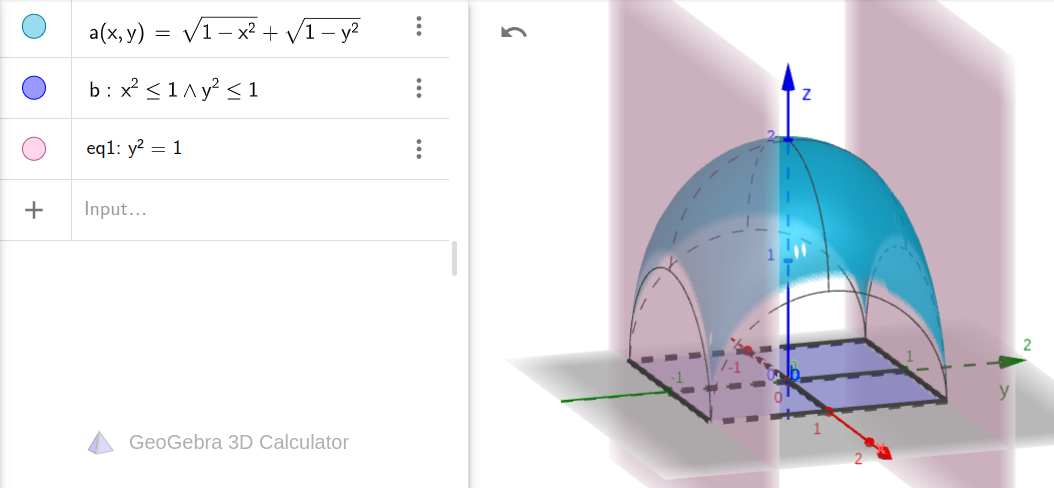
\includegraphics[width=\textwidth]{curva-di-livello-2.png}
\end{center}

Quindi il dominio \(D\) è chiuso.

\pagebreak
\subsubsection*{Esempio 3}

Determinare l'insieme di definizione della seguente funzione:

\[
    z = \frac{1}{\sqrt{y-\sqrt{x}}}
\]

\[
    D=\{(x,y) \in \R^{2} \giventhat y-\sqrt{x}>0,\ x \ge 0\}
\]

Vuole dire che prendiamo solo i valori che stanno a destra dell'asse y e nel sopragrafico della seguente parabola.

\begin{center}
    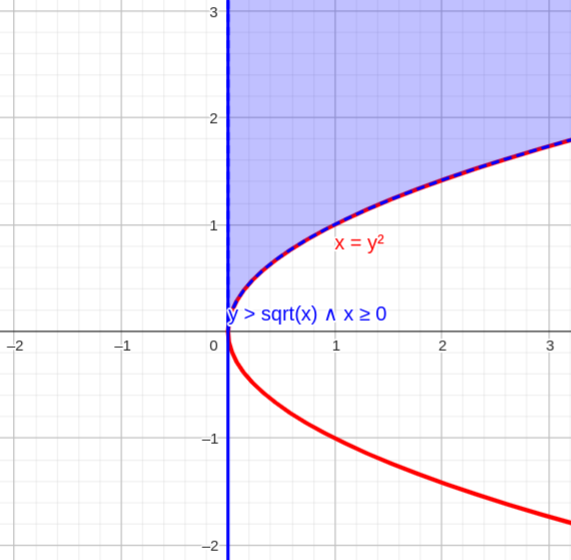
\includegraphics[width=0.65\textwidth]{curva-di-livello-3.png}
\end{center}

\pagebreak
\subsubsection{Esercizi {-} Insiemi di livello}

\subsubsection*{Esercizio 1}

Determinare gli insiemi di livello della seguente funzione:

\[
    z = x+2y
\]

Il dominio è tutto \(\R^2\).

\[
    E_k = \{(x,y) \in \R^2 \giventhat x+2y = k\} = \left\{(x,y) \in \R^2 \giventhat[\bigg] y = \frac{k-x}{2}\right\} \to \text{fascio di rette}
\]

\filbreak{}
\subsubsection*{Esercizio 2}

Determinare gli insiemi di livello della seguente funzione:

\[
    z = x^{2}+9y^{2}
\]

Il dominio è tutto \(\R^2\).

\[
    E_k = \{(x,y) \in \R^{2}\ \vert\ x^{2}+9y^{2}=k\}
\]

se \(k<0\): \(E_k = \emptyset \)

se \(k=0\): \(E_0=(0,0)\) ovvero l'origine degli assi

se \(k>0\): otteniamo delle ellissi:

\[
    \frac{x^{2}}{9}+ y^{2} = \frac{k}{9}
\]

\filbreak{}
\subsubsection*{Esercizio 3}

Determinare gli insiemi di livello della seguente funzione:

\[
    z= \frac{y}{x^{2}}
\]

dominio:

\[
    E_k = \left\{(x,y) \in \R^{2} \giventhat[\Big] x \neq  0;\ \frac{y}{x^{2}}=k \right\}
\]

se \(k=0\), è \(E_0\) privata dell'origine:

\[
    \frac{y}{x^{2}}=0
\]

se \(k \ne 0\):

\[
    \frac{y}{x^{2}} = k
\]

\[
    y = kx^{2}
\]

\vspace{5mm}
\begin{center}
    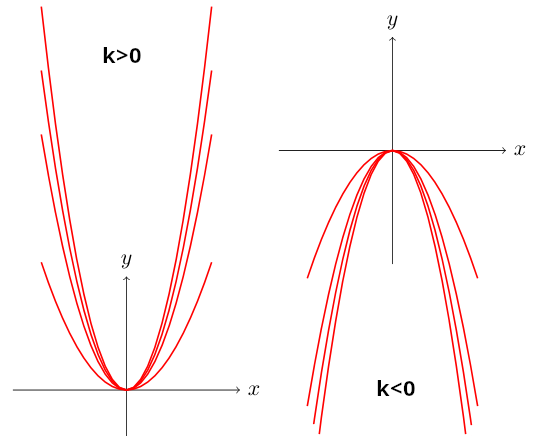
\includegraphics[width=0.6\textwidth]{insiemi-di-livello-esempio-4.png}
\end{center}

\filbreak{}
\subsubsection*{Esercizio 4}

Studiare gli insiemi di livello della seguente funzione:

\[
    z = \frac{2x}{x^2+y^2}
\]

Notiamo le condizioni di esistenza del denominatore:

\[f(x,y) = x^2 + y^2 \to f: \R^2 \setminus \{\uzero \} \to \R \]

Per cui gli insiemi di livello sono:

\[E_k = \left\{ (x,y) \in \R^2 \setminus \{(0,0)\} \giventhat[\bigg] \frac{2x}{x^2+y^2} = k \right\} \]

Se \(k=0\):

\[
    \frac{2x}{x^2+y^2} = 0 \implies x = 0;\ y \ne 0 \qquad \text{ovvero tutti i punti sull'asse \(y\) eccetto l'origine.}
\]

Se \(k \ne 0\):
\begin{align*}
    \frac{2x}{x^2+y^2} = k & \implies 2x = k (x^2+y^2) \implies kx^2 + ky^2 -2x = 0                                                        \\
                           & \implies x^2 + y^2 -\frac{2}{k}x = 0 \implies {\left( x-\frac{1}{k} \right)}^2 + y^2 = \frac{1}{k^2}          \\
                           & \text{ovvero le circonferenze di centro } c=\left( \frac{1}{k}, 0 \right) \text{ e raggio } r = \frac{1}{|k|}
\end{align*}
\begin{center}
    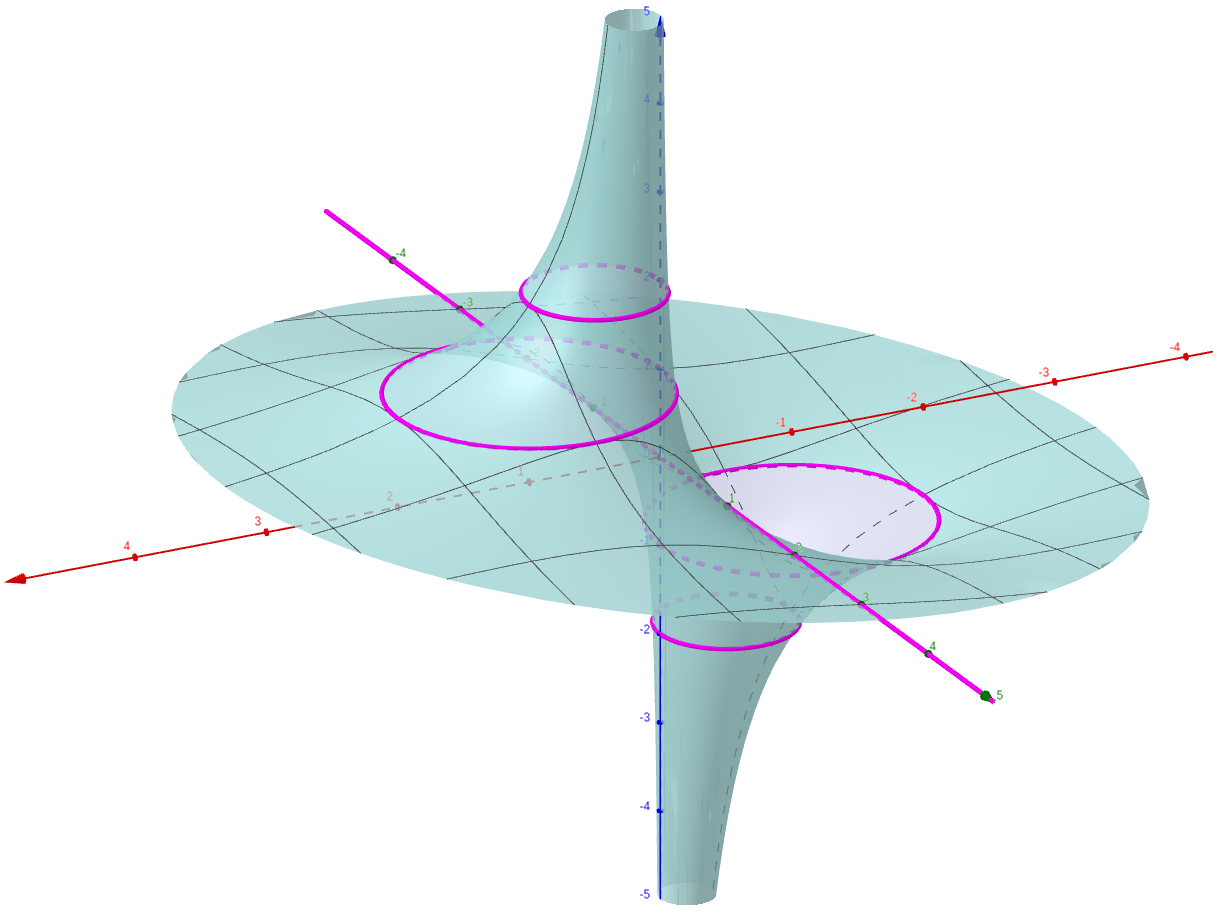
\includegraphics[width=0.7\textwidth]{insiemi-di-livello-esempio-5.png}
\end{center}

\pagebreak
\subsubsection{Esercizi {-} limiti}

\subsubsection*{Esercizio 1}

\[
    \lim_{ (x,y) \to (0,0) } \frac{xy(2y^{2}+x^{3})}{x^{4}+y^{2}}
\]

Sostituendo \((x,y)\) con \((0,0)\) otteniamo una forma indeterminata.

Consideriamo dunque le restrizione della funzione lungo le rette \(y=mx\):

\[
    \lim_{\begin{smallmatrix}(x,y) \to (0,0) \\ y=mx\end{smallmatrix}} f(x,y) = \lim_{\begin{smallmatrix}(x,y) \to (0,0) \\ y=mx\end{smallmatrix}} \frac{xmx(2m^{2}x^{2}+x^{3})}{x^{4}+m^{2}x^{2}}= \lim_{ x \to 0 } \frac{mx^{2}(2m^{2}+x)}{(x^{2}+m^{2})} = 0
\]

il limite quindi se esiste deve essere zero. Passiamo adesso alle coordinate polari per valutare \(f\):

\begin{spreadlines}{3mm}
    \begin{align*}
        \left|f(\rho, \theta)\right| & = \left|\frac{\rho\cos(\theta) \rho\sin(\theta) (2\rho^{2}\sin^{2}(\theta)+\rho^{3}\cos^{3}(\theta))}{\rho^{4}\cos^{4}(\theta)+\rho^{2}\sin^{2}(\theta)}\right| \\
                                     & = \left|\frac{\rho^{2}\cos(\theta) \sin(\theta) (2\sin^{2}(\theta)+\rho \cos^{2}(\theta))}{\rho^{2}\cos^{4}(\theta)+\sin^{2}(\theta)} \right|                   \\
                                     & \le \left|\rho^{2}\cos(\theta) \sin(\theta) (2\sin^{2}(\theta)+\rho \cos^{2}(\theta))\right|                                                                    \\
                                     & = \left|2\rho^{2}\cos(\theta)\sin^3(\theta) + \rho^{3}\cos^3(\theta)\sin(\theta)\right|                                                                         \\
                                     & \le 2\rho^2|\cos(\theta)\sin^3(\theta)| + \rho^2|\rho\cos^3(\theta)\sin(\theta)|                                                                                \\
                                     & \le 2\rho^2 + \rho^4 \xrightarrow[\rho \to 0^+]{} 0
    \end{align*}
\end{spreadlines}

Il limite di \(f(x,y)\) per \((x,y) \to (0,0)\) dunque esiste e vale \(0\).

Per dimostrarlo, potevamo usare anche un altro metodo senza passare alle coordinate polari:

\[
    \left|f(x,y)\right| =  \left|\frac{xy(2y^{2}+x^{3})}{x^{4}+y^{2}}\right| = \left|\frac{2xy^{3}+x^{4}y}{x^{4}+y^{2}}\right| = \left| \frac{2xy^{3}}{x^{4}+y^{2}}+ \frac{x^{4}y}{x^{4}+y^{2}}\right| \le \left|\frac{2xy^{3}}{x^{4}+y^{2}}\right|+ \left|\frac{x^{4}y}{x^{4}+y^{2}}\right|
\]

quindi:

\[
    |f(x,y)|  \le \frac{2|xy^{3}|}{x^{4}+y^{2}} + \frac{x^{4}|y|}{x^{4}+y^{2}} \le \frac{2|xy^{3}|}{y^{2}} + \frac{x^{4}|y|}{x^{4}}
\]

\[
    |f(x,y)|  \le \underbrace{2 |xy| + |y|}_{g(x,y)}
\]

La funzione \(g\) è continua su tutto \(\R \) ed è inoltre \(\ge 0\). Dunque, il limite è:

\[
    \lim_{ (x,y) \to (0,0) } g(x,y) = g(0,0) = 0
\]

Quindi per il teorema del confronto, 0 è effettivamente il limite di \(f(x,y)\) per \((x,y) \to (0,0)\)

\filbreak{}
\subsubsection*{Esercizio 2}

\[
    \lim_{ (x,y) \to (0,0) } \frac{x\sin^{2}(y)+ 3xy^{4}}{x^{2}+2y^{4}}
\]

Sostituendo \((x,y)\) con \((0,0)\) otteniamo una forma indeterminata.

riscrivo la \(f\) come somma di due funzioni:

\[
    f(x,y) = \frac{x\sin^{2}(y)+ 3xy^{4}}{x^{2}+2y^{4}}  = \underbrace{\frac{x\sin^{2}(y)}{x^{2}+2y^{4}}}_{f_1(x,y)} + \underbrace{\frac{3xy^{4}}{x^{2}+2y^{4}}}_{f_2(x,y)}
\]

Affinché \(f(x,y)\) abbia limite, anche \(f_1, f_2\) devono averlo.

Vediamo prima \(f_2\) che è più semplice.

\[
    |f_2(x,y)| = \left| \frac{3xy^{4}}{x^{2}+2y^{4}}\right| =\frac{3y^{4}|x|}{x^{2}+2y^{4}} \le \frac{3y^{4}|x|}{2y^{4}} = \frac{3}{2}|x| \rightarrow 0
\]

Dunque, \(f_2(x,y) \xrightarrow[(x,y) \to (0,0)]{} 0\).

Vediamo ora \(f_1\):

\[
    f_1(x,y) = \frac{x\sin^{2}y}{x^{2}+2y^{4}}
\]

Notiamo che se passiamo alle coordinate polari, il numeratore va come \(\rho^{3}\), mentre il denominatore come \(\rho^{4}\). Il limite potrebbe quindi non esistere, controlliamolo.

Ricordando che \(\sin(x) \xrightarrow[x \to 0]{} 0\);

Guardo la funzione lungo il cammino \(y=x\):

\[
    \lim_{ \begin{smallmatrix}(x,y) \to (0,0) \\ y=x \end{smallmatrix} } f_1(x,y) = \lim_{ x \to 0 } \frac{x\sin^{2}(x)}{x^{2}+2x^{4}} = \lim_{ x \to 0 } \frac{x\sin^{2}(x)}{x^{2}(1+2x^{2})} = \lim_{ x \to 0 } \frac{x}{1+2x^2} = 0
\]

Per \(x = y^{2}\):

\[
    \lim_{ \begin{smallmatrix}(x,y) \to (0,0) \\ x=y^2 \end{smallmatrix} } f_1(x,y)  = \lim_{ y \to 0 } \frac{y^{2}\sin^{2}(y)}{y^{4}+2y^{4}} = \lim_{ y \to 0 } \frac{\sin^{2}(y)}{3y^{2}}  = \frac{1}{3}
\]

quindi il limite non esiste perché \(f= f_1+f_2\) ma \(\lim_{ (x,y) \to (0,0) } f_1\) non esiste.

\pagebreak
\subsubsection{Scelta delle curve di restrizione}

Nell'esercizio di prima come ho fatto a restringere la \(f_1\)?

Vediamolo:

\begin{itemize}
    \item \(y=x\), peso le variabili allo stesso modo e dunque dal denominatore (\(x^{2}+2y^{4}\)) ottengo \(x^{2}+2x^{4}\). Quindi, per \(x \rightarrow 0\), sto dando più importanza al monomio \(x^2\).
    \item \(x=y^{2}\), dal denominatore (\(x^{2}+2y^{4}\)) ottengo \(y^{4}+2y^{4} = 3y^{4}\) quindi qua non trascuro gli addendi che ora hanno lo stesso peso.
\end{itemize}

In generale, quindi, quando si cerca di verificare la \textbf{NON ESISTENZA} del limite, si prova a vedere cosa fa la funzione dando pesi diversi alle vari parti che la compongono.

\subsubsection*{Esempio}

\[
    \lim_{ (x,y) \to (0,0) } \left( \left( \frac{xy^{2}+2y^{ \frac{1}{3}}\sin^{2}(x)}{x^{2}+y^{2}}\right) \cdot e^{ \left(\frac{x^{2}-y^{2}}{x^{2}+y^{2}}\right)} \right)
\]

L'esponente dell'esponenziale, preso da solo, abbiamo già verificato che non ha limite. Se però riusciamo a dimostrare che esiste il limite per la prima parentesi, e inoltre riusciamo a limitare uniformemente l'esponenziale, allora abbiamo un limite per il tutto.

Vediamo l'esponente dell'esponenziale:

\[
    \frac{x^{2}-y^{2}}{x^{2}+y^{2}} \le \left|\frac{x^{2}-y^{2}}{x^{2}+y^{2}}\right| = \frac{\left|x^{2}-y^{2}\right|}{x^{2}+y^{2}}  \le \frac{\left|x^{2}\right|+\left|y^{2}\right|}{x^{2}+y^{2}} = \frac{x^{2}+y^{2}}{x^{2}+y^{2}} = 1
\]
quindi:
\[
    0 < e ^{ \frac{x^{2}-y^{2}}{x^{2}+y^{2}}} \le e
\]

Buono, a noi non da noia che sta tra \(0\) ed \(e\), ci importa solo che il limite esiste e non tende all'infinito.

Studiamo ora l'altra parte della funzione \(f(x,y)\) usando le coordinate polari:

\begin{align*}
    \left| \frac{\rho\cos(\theta) \rho^{2}\sin^{2}(\theta) + 2 \rho^{\frac{1}{3}}\sin^{\frac{1}{3}}(\theta) \sin^{2}(\rho\cos(\theta))}{\rho^{2}}\right| & \le \left| \frac{\rho^{3}\cos(\theta)\sin^{2}(\theta)}{\rho^{2}}\right| + \left|\frac{2 \rho^{\frac{1}{3}}\sin^{\frac{1}{3}}(\theta) \sin^{2}(\rho\cos(\theta)) }{\rho^{2}}\right| \\
                                                                                                                                                         & \le \left| \rho\cos(\theta) \sin ^{2}(\theta)\right| + \left|\frac{2 \rho^{\frac{1}{3}} \sin^{\frac{1}{3}}(\theta) \rho^2\sin^{2}(\cos(\theta)) }{\rho^{2}}\right|                 \\
                                                                                                                                                         & \le \left| \rho\cos(\theta) \sin ^{2}(\theta)\right| + \left| 2 \rho^{\frac{1}{3}} \sin^{\frac{1}{3}}(\theta) \sin^{2}(\cos(\theta)) \right|                                       \\
                                                                                                                                                         & \le \left| \rho\cos(\theta) \sin ^{2}(\theta)\right| + 2 \rho^{ \frac{1}{3}} \left| \sin^{\frac{1}{3}}(\theta) \cos^{2}(\theta)\right|                                             \\
                                                                                                                                                         & \le \rho + 2 \rho^{ \frac{1}{3}} \xrightarrow[\rho \to 0^+]{} 0
\end{align*}

quindi alla fine il limite è:

\[
    \lim_{ (x,y) \to (0,0) } f(x,y) = 0 \cdot e = 0
\]


\end{document}
